\documentclass[11pt]{article}

\usepackage[margin=1in]{geometry}
\usepackage{amsmath}
\usepackage{booktabs}
\usepackage{enumitem}
\usepackage{listings}
\usepackage{tikz}
\usetikzlibrary{arrows.meta, calc, fit, positioning}
\usepackage[hidelinks]{hyperref}

\lstset{basicstyle=\small\ttfamily, columns=fullflexible, keepspaces=true}
\newcommand{\code}[1]{\texttt{#1}}

\tikzset{
  box/.style={draw, rounded corners, minimum height=0.8cm, align=center, font=\small},
  arrow/.style={-{Stealth}, thick},
  subscription/.style={-{Stealth}, thick, dashed},
  lbl/.style={font=\footnotesize, midway, above},
}

\title{Gabriel: Compute DAGs and Token Flow}
\author{Design note}
\date{\today}

\begin{document}
\maketitle
\tableofcontents
\newpage

\section{Introduction}

Gabriel sends inputs, such as camera frames, from \emph{producers} on a device
to \emph{engines} that process them. It then sends the engines' results back.
Today, each input makes a single hop from a producer to the engines that
consume it. This note extends Gabriel to \emph{flows}: an input can pass
through a DAG of engines, some on the device and some on a cloudlet.

\subsection{Gabriel today}

\paragraph{Tokens.} Gabriel uses tokens to limit how many frames are in
flight. A producer can only send a frame while it holds a token, and the token
comes back once the frame has been processed. When the network or the engines
slow down, tokens come back more slowly, so the producer sends fewer frames.
Frames that could not be processed in time are never sent, so they waste no
bandwidth.

\paragraph{Fastest consumer.} When several engines consume the same producer,
Gabriel sends frames as fast as the \emph{fastest} engine can process them.
The server gives each frame to every engine that consumes the producer. It
returns the token as soon as the \emph{first} engine finishes, and a flag
(\code{pending\_token\_return} in \code{server\_runner.py}) stops later
engines from returning it again. A slower engine never falls behind: when it
becomes
free while a frame is in flight, it takes that frame and skips the ones it
missed. If an engine asks for all its results, its results are sent back even
when it finishes after the first engine.

\subsection{Patterns to support}

The SteelEagle DDIL paper uses two very different techniques. The DAG must
support both:
\begin{itemize}[nosep]
  \item \textbf{Early discard} (filtered edge offload): an engine on the
        device filters frames, and only the frames that pass are sent to the
        cloudlet. The engines run \emph{in series}.
  \item \textbf{Multi-tier fusion}: engines on the device and on the
        cloudlet process the same frames \emph{in parallel}, and a fusion
        engine combines their results. The fast result from the device can
        trigger a speculative action, which the slower but definitive result
        from the cloudlet then confirms or cancels.
\end{itemize}
Either technique can be extended with \textbf{feedback}: a local engine
subscribes to a remote engine's results, and uses them to update its own
state. For example, in early discard with a local PatchCore anomaly detector,
PatchCore forwards suspected anomalies to a remote verifier. When the
verifier says an anomaly was a false positive, PatchCore adds that frame's
features to its memory bank, so that it stops flagging similar frames. This
is a form of the paper's dynamic terrain adaptation, in which cloudlet AI
teaches on-device AI. Section~\ref{sec:overview} gives an example with all
three, and Section~\ref{sec:examples} works through each in detail.

The paper also relies on two features for disconnected operation, which
Section~\ref{sec:disconnected} covers:
\begin{itemize}[nosep]
  \item \textbf{Prioritized reintegration}: while the device is disconnected
        or weakly connected, the app records every frame and queues requests
        for cloudlet AI. When connectivity returns, it sends the most
        important ones first, and each is processed exactly once.
  \item \textbf{Reachback}: a cloudlet engine asks the device for specific
        recorded frames, e.g.\ the frames around a place where on-device AI
        may have missed something, and processes them with its better models.
\end{itemize}

\subsection{Goals}

The design must:
\begin{enumerate}[nosep]
  \item limit how many frames from each producer are in flight, counting the
        whole path through the DAG;
  \item send frames as fast as the fastest path can process them, while
        slower engines skip to the newest frame instead of falling behind;
  \item send a frame to the cloudlet only when the cloudlet will process it
        soon, so that frames do not pile up on the network or at the
        cloudlet;
  \item return a token as soon as a frame's processing finishes, including
        when an engine discards it, and return each token exactly once, even
        when messages are duplicated, retried, or lost;
  \item route frames through several engines on the device and on the
        cloudlet, with frames moving only from the device to the cloudlet and
        only results coming back;
  \item let any process, an engine or the app, see every result of the
        engines it cares about, and learn when a result will not come;
  \item keep on-device processing running while the cloudlet is unreachable,
        and let the app send recorded frames later, in its own priority order
        or when the cloudlet asks for them, with each one processed exactly
        once.
\end{enumerate}
Goals 1 to 3 serve one objective, which the next section states.

\subsection{What to optimize}
\label{sec:objective}

\paragraph{Waiting is the cost.} The time from capturing a frame to getting
its result has three parts:
\begin{itemize}[nosep]
  \item \textbf{processing}: the time the frame spends in engines;
  \item \textbf{transit}: the time it spends on the network;
  \item \textbf{waiting}: all the rest. The frame waits for a token, in a
        pending slot, or in a queue.
\end{itemize}
Processing and transit are the price of the work. Waiting is what Gabriel
adds, so Gabriel should keep it small.

\paragraph{Throughput matters as much.} An engine that sits idle does not
add waiting, but its results come less often. A result that never comes is
the stalest of all. So the objective is to keep waiting small \emph{while}
keeping the slowest engine on each path busy.

\paragraph{One number for both: the age of information.} At each moment, the
age of an app's newest result is the time since the frame behind it was
captured. Its average over time is the \emph{age of information} (AoI). It
grows with waiting, because results arrive older. It also grows when results
are rare, because the newest one gets old before the next arrives. For
results that come at a steady pace, the average age is about the latency plus
half the time between results. AoI is the main measure of the evaluation
(\code{docs/evaluation.tex}); waiting and engine use explain it.

\paragraph{The trade-off.} Take any place where an input can wait in front of
an engine. When the engine becomes free, one of three things is true:
\begin{itemize}[nosep]
  \item \textbf{No input is there.} The engine sits \emph{idle}: throughput
        is lost.
  \item \textbf{An old input is there}, and nothing can replace it. The
        engine starts on it late: \emph{waiting} is added.
  \item \textbf{A fresh input is there}, because newer inputs kept replacing
        older ones. The replaced inputs were moved, and maybe processed
        upstream, for nothing: this is \emph{waste}.
\end{itemize}
Only an input that arrives exactly when the engine becomes free avoids all
three. Engine times vary, so this needs luck or a good prediction. Every
mechanism therefore picks which cost to pay:
\begin{center}
\small
\begin{tabular}{@{}llll@{}}
\toprule
Mechanism & Waiting & Idle & Waste \\
\midrule
Queue in front of the engine (FIFO) & grows with load & none & none \\
Fetch an input when the engine is free & none & one fetch time & none \\
Keep the slot supplied, newest wins & small & none & skipped inputs \\
\bottomrule
\end{tabular}
\end{center}
How much each cost weighs depends on where the engine is:
\begin{itemize}[nosep]
  \item \textbf{On the device}, a fetch takes about 0.1\,ms and a copy is
        cheap. Fetching and keeping slots supplied both work well. The waste
        that matters is \emph{compute}: an upstream engine that processes
        inputs a downstream engine later skips. Engines on a device share
        its CPU and GPU, so that waste can slow the bottleneck.
  \item \textbf{On the cloudlet}, a fetch takes a network round trip, often
        as long as the processing itself, and waste costs bandwidth. Here the
        trade-off is real, and the right point depends on the link.
\end{itemize}
Gabriel keeps each slot supplied with newest-wins pending slots
(\S\ref{sec:edges}), and limits how much it sends with tokens and crossing
capacities. \S\ref{sec:alternatives} asks whether those are the right limits.

\paragraph{In queueing terms.} The evaluation uses these terms, per engine:
\begin{itemize}[nosep]
  \item the \textbf{arrival rate} $\lambda$: offers made to the engine per
        second, and its \textbf{service time} $S$: how long it takes per
        input;
  \item the \textbf{offered load} $\rho = \lambda \cdot E[S]$. Above 1,
        more candidates arrive than the engine can serve, and the rest are
        skipped. That is the price of always having a fresh one, not a fault;
  \item the \textbf{utilization} $U$: the share of time the engine is busy.
        This is the throughput side;
  \item \textbf{Little's law}, $L = \lambda W$: the average number of inputs
        in a part of the system is its arrival rate times the time each one
        spends there. Applied to a producer, it gives how many tokens are in
        use on average.
\end{itemize}
A producer's tokens make a \emph{closed} system: a fixed number of inputs
circulate. Its throughput rises with the token count up to a \emph{knee},
\[
  N^* = \frac{\text{time an input spends on the whole path, network
  included}}{\text{service time of the slowest engine}},
\]
and stays flat after it. In a FIFO system, every input above the knee adds
one service time of the slowest engine to the waiting. The best balance of
throughput and delay is at the knee; this is the point that TCP's BBR aims
for. With newest-wins slots, inputs above the knee are skipped instead, so
they add waste, not waiting. Analyses of queues that keep only the newest
waiting update (Costa, Codreanu, and Ephremides, 2016) find them fresher than
FIFO for the same reason.

\section{Overview}
\label{sec:overview}

This section gives the whole design in brief. Later sections describe each
part in detail.

\subsection{Three building blocks}

\begin{description}[style=nextline, leftmargin=1.5em]
  \item[Producers create inputs.] A producer publishes inputs, such as camera
        frames, on an iceoryx2 service, and gives each input an id. Most
        producers are separate processes. Some live inside the client, e.g.\ a
        \emph{telemetry} producer that publishes bandwidth and round-trip
        estimates. Downstream, all producers are treated the same.
  \item[Flows bound and route work.] A flow carries a producer's inputs through
        a DAG of engines, some on the device and some on the cloudlet. Flows
        are \emph{token-gated and newest-wins}: the producer sends inputs as
        fast as the fastest path can process them, a slower engine skips to the
        newest input instead of falling behind, and an input that cannot be
        sent in time is dropped rather than queued. Use a flow whenever work
        must be bounded and fresh inputs matter more than complete ones.
  \item[Event services report what happened.] Each machine publishes the
        events of its engines on iceoryx2: an input was sent to an engine,
        finished with a result, skipped, or timed out. Any process can
        \emph{subscribe}: an engine such as a fusion engine, the producer's
        app, or a monitoring tool. A subscriber gets \emph{every} event, in
        order, from a buffer of fixed size. Use a subscription whenever a
        consumer must not miss anything, including the news that a result will
        not come.
\end{description}

The two delivery mechanisms are deliberately different. Flows drop inputs on
purpose, to stay fresh and bounded; event services never drop events on
purpose, so that subscribers can match results for the same input.

\subsection{Processes}

\begin{figure}[h]
\centering
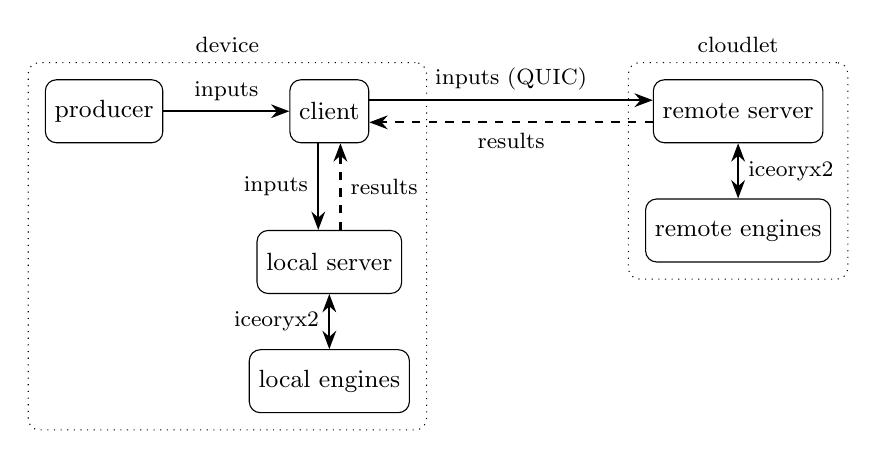
\begin{tikzpicture}[node distance=0.7cm and 1.6cm]
  \node[box] (prod) {producer};
  \node[box, right=of prod] (client) {client};
  \node[box, below=1.1cm of client] (ls) {local server};
  \node[box, below=of ls] (le) {local engines};
  \node[box, right=3.6cm of client] (rs) {remote server};
  \node[box, below=of rs] (re) {remote engines};
  \draw[arrow] (prod) -- node[lbl] {inputs} (client);
  \draw[arrow] ([xshift=-4pt]client.south) -- node[font=\footnotesize, midway, left] {inputs} ([xshift=-4pt]ls.north);
  \draw[subscription] ([xshift=4pt]ls.north) -- node[font=\footnotesize, midway, right] {results} ([xshift=4pt]client.south);
  \draw[{Stealth}-{Stealth}, thick] (ls) -- node[font=\footnotesize, midway, left] {iceoryx2} (le);
  \draw[{Stealth}-{Stealth}, thick] (rs) -- node[font=\footnotesize, midway, right] {iceoryx2} (re);
  \draw[arrow] ([yshift=4pt]client.east) -- node[lbl] {inputs (QUIC)} ([yshift=4pt]rs.west);
  \draw[subscription] ([yshift=-4pt]rs.west) -- node[font=\footnotesize, midway, below] {results} ([yshift=-4pt]client.east);
  \node[draw, dotted, rounded corners, inner sep=6pt, fit=(prod) (client) (ls) (le),
        label={[font=\footnotesize]above:device}] {};
  \node[draw, dotted, rounded corners, inner sep=6pt, fit=(rs) (re),
        label={[font=\footnotesize]above:cloudlet}] {};
\end{tikzpicture}
\caption{The client connects to two servers that run the same code: a local
server on the device, reached over iceoryx2, and a remote server on the
cloudlet, reached over QUIC. Inputs go from the client to the servers; only
results come back.}
\label{fig:arch}
\end{figure}

\begin{description}[nosep]
  \item[Producers] publish inputs on iceoryx2 services.
  \item[The client] subscribes to its producers and keeps the newest input
        from each. It connects to one local server and one remote server, and
        sends each input to the server whose engines should process it. It
        owns all the tokens.
  \item[The local and remote servers] run the same program, once on the
        device and once on the cloudlet. Each server talks to its engines over
        iceoryx2, accepts clients, and routes inputs between its engines. The
        two differ only in how clients reach them: over iceoryx2 for the local
        server, and over QUIC for the remote server.
  \item[Engines] use the same engine ABI on both servers. An engine does not
        know whether it runs on the device or on the cloudlet, so moving an
        engine between them only changes the flow spec, not the engine.
\end{description}


\subsection{An example}

A drone looks for vehicles with two detectors, and for anomalies with
PatchCore:

\begin{figure}[h]
\centering
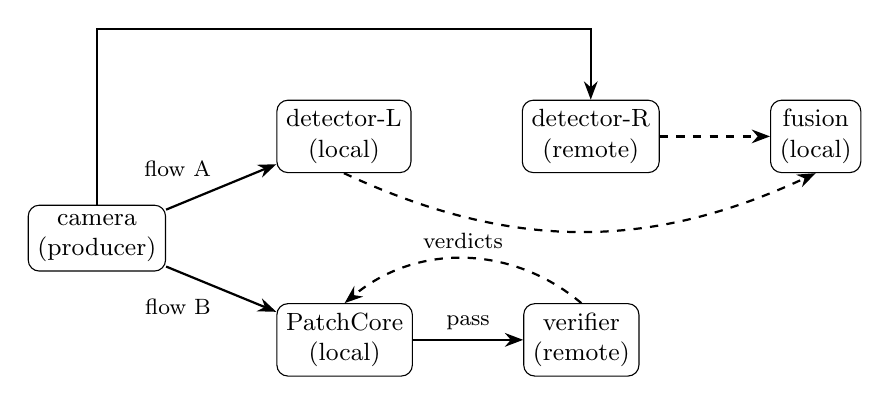
\begin{tikzpicture}[node distance=0.5cm and 1.4cm]
  \node[box] (cam) {camera\\(producer)};
  \node[box, above right=0.4cm and 1.4cm of cam] (dl) {detector-L\\(local)};
  \node[box, right=of dl] (dr) {detector-R\\(remote)};
  \node[box, right=of dr] (fusion) {fusion\\(local)};
  \node[box, below right=0.4cm and 1.4cm of cam] (pc) {PatchCore\\(local)};
  \node[box, right=of pc] (ver) {verifier\\(remote)};
  \draw[arrow] (cam) -- node[font=\footnotesize, midway, above left] {flow A} (dl);
  \draw[arrow] (cam.north) |- ([yshift=0.9cm]dl.north) -| (dr.north);
  \draw[arrow] (cam) -- node[font=\footnotesize, midway, below left] {flow B} (pc);
  \draw[arrow] (pc) -- node[lbl] {pass} (ver);
  \draw[subscription] (dl.south) to[bend right=25] (fusion.south);
  \draw[subscription] (dr) -- (fusion);
  \draw[subscription] (ver.north) to[bend right=40] node[font=\footnotesize, midway, above] {verdicts} (pc.north);
\end{tikzpicture}
\caption{Solid arrows are flows; dashed arrows are subscriptions to event
services. Flow A feeds both detectors; fusion subscribes to both detectors'
events. Flow B is early discard; PatchCore subscribes to the verifier's
verdicts.}
\label{fig:overview}
\end{figure}

\paragraph{Flow A and fusion.} Detector-L takes 0.1~s per frame, detector-R
0.3~s including the network, and the camera has one token in flow A.
\begin{enumerate}[nosep]
  \item Frame 42 is admitted and sent to both detectors. The event services
        publish that 42 was sent to each.
  \item At 0.1~s, detector-L reports its result for 42. This is the frame's
        first completion, so its token returns. Fusion reads the result. It
        also knows detector-R has frame 42, so it can start a speculative
        action and wait for the definitive result.
  \item Frame 43 is admitted at once and sent to detector-L. Detector-R is
        still busy, so 43 waits in its pending slot.
  \item At 0.2~s, detector-L finishes 43 and frame 44 is admitted. Frame 44
        replaces 43 in detector-R's pending slot, which publishes that 43 was
        skipped for detector-R. Fusion acts on detector-L's result for 43 right
        away, instead of waiting for a remote result that will never come.
  \item At 0.3~s, detector-R reports its result for 42. Fusion matches it with
        detector-L's result for 42, and confirms or cancels its speculative
        action. Detector-R then takes frame 44, which detector-L also processed.
\end{enumerate}
Flow A decides the \emph{work}: it runs at detector-L's speed and sends
detector-R only frames that detector-L also processed. Fusion's subscription
decides what fusion \emph{knows}: it sees every event, including the ``skipped''
that tells it not to wait.

\paragraph{Flow B and feedback.} PatchCore reports a normal frame as finished,
which returns its token, and passes a suspected anomaly on to the verifier,
keeping the frame's patch features. When the verifier says an anomaly was a
false positive, PatchCore reads that verdict from its subscription between
frames, and adds the features to its memory bank.

\paragraph{Telemetry.} The client's bandwidth producer publishes an estimate
every second. The app subscribes to it, and raises PatchCore's threshold when
bandwidth drops: the paper's bandwidth adaptation.

\subsection{How the design guarantees this}

\begin{itemize}[nosep]
  \item \textbf{Tokens are end-to-end.} An input keeps its token along its
        whole path and returns it at its first completion, so the producer
        adapts to the network and to every engine on the fastest path
        (\S\ref{sec:tokens}).
  \item \textbf{Edges bound queues.} Each edge has a capacity and one pending
        slot, so a slow engine never builds a backlog (\S\ref{sec:edges}).
  \item \textbf{The client owns all tokens.} The servers forward inputs between
        their own engines, and report every event to the client, which tracks
        each input with a ticket (\S\ref{sec:accounting}).
  \item \textbf{Every offer ends with exactly one event}, so a token returns
        exactly once, and subscribers always learn whether a result can still
        come (\S\ref{sec:events}).
\end{itemize}

\section{Concepts}
\label{sec:concepts}

This section defines each concept briefly. Later sections describe them in
detail.

\begin{description}[style=nextline, nosep, leftmargin=1.5em]
  \item[Flow] A named DAG of producer and engine nodes connected by edges. A
        client registers a flow with \code{add\_flow(name, spec)}.
  \item[Producer node] A source of inputs, such as a camera. Producers have
        no incoming edges, so they are always roots of the DAG. A \emph{live}
        producer publishes frames as they are captured, and Gabriel takes the
        newest one whenever it has room. An \emph{on-demand} producer waits
        until Gabriel says it has room, then chooses what to send, e.g.\ the
        most important recorded frame (\S\ref{sec:disconnected}).
  \item[Engine node] Processes inputs, one at a time. A \emph{local} engine
        runs on the device; a \emph{remote} engine runs on the cloudlet.
  \item[Input] A frame, or the data an engine produced from a frame. Each
        input has an \code{InputId}, and a payload type that says how to read
        its bytes.
  \item[Input edge] Carries inputs from a producer or an engine to another
        engine. Edges always end at an engine, since producers have no
        incoming edges. A node can have
        several incoming edges (fan-in) and several outgoing edges (fan-out).
        A \emph{branch} is one outgoing edge of a fan-out, together with
        everything after it.
  \item[Outcome] What an engine reports for each input. It has an optional
        \emph{result} and a \emph{forward} decision: \code{Pass} forwards the
        input unchanged, \code{Emit} forwards a new input (such as the tiles of
        a frame), and \code{Stop} forwards nothing.
  \item[Completion] An input completes along a path when an outcome forwards
        it to no edge. This happens on \code{Stop}, or on \code{Pass} or
        \code{Emit} from an engine that has no outgoing input edges in the
        flow.
  \item[Token] Each producer of a flow has a pool of $C$ tokens. An input
        needs a token to enter the flow. It keeps the token along its whole
        path (the token is \emph{end-to-end}), and the token returns when the
        input first completes.
  \item[Offer] One input offered to one input edge. If the edge has spare
        \emph{capacity}, the offer is sent. Otherwise it waits in the edge's
        \emph{pending slot}, which holds one offer; a newer offer replaces it.
        An offer \emph{ends} when the engine at the end of its edge is done
        with it, which is about that one edge, not the input's whole path.
  \item[Crossing] A group of edges that the client sends inputs along to
        one server. When a node feeds several engines on the same server, the
        client groups its edges to them into one crossing, so that each input
        is sent to that server only once.
  \item[Result event] A message that says what happened to an offer: it was
        sent, finished with a result, skipped, or timed out. Every offer ends
        in exactly one such event, so subscribers always know whether a result
        can still come.
  \item[Event service] An iceoryx2 service on which an engine's result events
        are published, on the machine where the engine runs, and on the device
        for remote engines. Any process can \emph{subscribe} to it.
  \item[Ticket] The client's record of an input it admitted. It lists the
        input's offers that have not ended, and whether the input still holds
        its token.
\end{description}

\paragraph{The life of an input.} A producer publishes a frame. If the
flow has a token for that producer, the client admits the frame and opens a
ticket for it. The frame is then offered to each of the producer's outgoing
edges. On each edge, it is either sent to the engine or, if the engine is
busy, kept in the edge's pending slot. Each engine that receives the frame
reports an outcome. If the outcome forwards the frame, the frame is offered to
that engine's outgoing edges, which may lead to the cloudlet. Otherwise, the
frame has completed along that path. Every step is reported as a result
event. The client uses these events to keep the ticket up to date, and returns
the token when the frame first completes. The events are also published on
the engines' event services, where the app and other engines read them.

\section{Architecture}
\label{sec:arch}

The processes are introduced in \S\ref{sec:overview}. This section describes
how a flow is split between them, and how it is installed.

\subsection{Local and remote parts}

\begin{figure}[h]
\centering
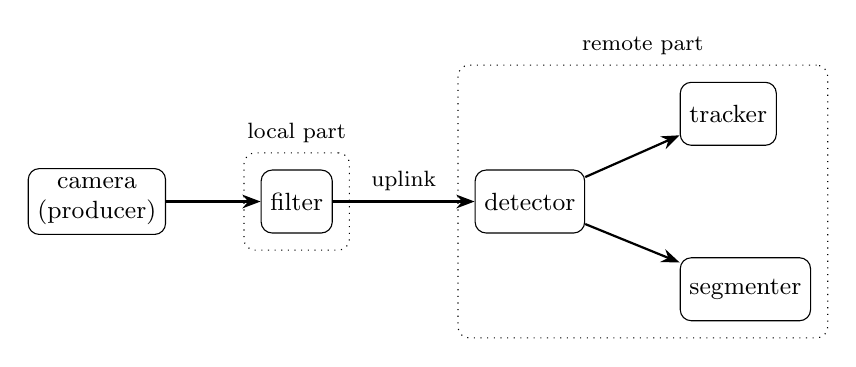
\begin{tikzpicture}[node distance=0.9cm and 1.2cm]
  \node[box] (cam) {camera\\(producer)};
  \node[box, right=of cam] (filter) {filter};
  \node[box, right=1.8cm of filter] (det) {detector};
  \node[box, above right=0.3cm and 1.2cm of det] (track) {tracker};
  \node[box, below right=0.3cm and 1.2cm of det] (seg) {segmenter};
  \draw[arrow] (cam) -- (filter);
  \draw[arrow] (filter) -- node[lbl] {uplink} (det);
  \draw[arrow] (det) -- (track);
  \draw[arrow] (det) -- (seg);
  \node[draw, dotted, rounded corners, inner sep=6pt, fit=(filter),
        label={[font=\footnotesize]above:local part}] {};
  \node[draw, dotted, rounded corners, inner sep=6pt, fit=(det) (track) (seg),
        label={[font=\footnotesize]above:remote part}] {};
\end{tikzpicture}
\caption{A flow split into a local and a remote part. Inputs cross from local
to remote only along uplink edges.}
\label{fig:parts}
\end{figure}

Each flow has a \emph{local part}, run by the local server, and a
\emph{remote part}, run by the remote server. Each part can contain several
engines. Inputs only move from local to remote: once an input reaches the
remote server, only results come back. An input edge from a local engine to a
remote engine is called an \emph{uplink}.

\code{add\_flow} rejects a flow whose input edges do not form a DAG, or that
has an edge the table below forbids:

\begin{center}
\small
\begin{tabular}{@{}ll@{}}
\toprule
Input edge & Allowed? \\
\midrule
producer $\to$ local or remote engine & yes \\
local $\to$ local engine   & yes \\
local $\to$ remote engine  & yes (an \emph{uplink}) \\
remote $\to$ remote engine & yes \\
remote $\to$ local engine  & no: only results come back \\
\bottomrule
\end{tabular}
\end{center}
Results come back to the device through event services (\S\ref{sec:subscribe}),
not through input edges.

\subsection{Who owns what}
\label{sec:ownership}

The app describes a flow as one graph, with the location of every engine. It
never says who owns what. Each input edge is owned by the process that has to
send inputs along it:

\begin{center}
\small
\begin{tabular}{@{}lll@{}}
\toprule
Edge & Owner & Why \\
\midrule
producer $\to$ any engine & client & the client receives producer frames \\
local $\to$ local engine & local server & both ends are on the local server \\
local $\to$ remote engine (uplink) & client & only the client is connected to the cloudlet \\
remote $\to$ remote engine & remote server & both ends are on the remote server \\
\bottomrule
\end{tabular}
\end{center}

In short: an edge between two engines on the same server belongs to that
server, and every other edge belongs to the client. For example, in a cascade
of filters,
\begin{center}
camera $\xrightarrow{\text{client}}$ motion (local)
$\xrightarrow{\text{local}}$ YOLO-n (local)
$\xrightarrow{\text{client}}$ YOLO-l (remote)
$\xrightarrow{\text{remote}}$ tracker (remote)
\end{center}
the local server forwards frames from the motion detector to YOLO-n by itself.
When YOLO-n passes a frame, its next edge belongs to the client, so the local
server only reports the \code{Pass}, and the client sends the frame to the
cloudlet. An engine can have outgoing edges of both kinds; then the server
forwards on its own edges and the client on its edges, for the same outcome.

\begin{itemize}[nosep]
  \item \textbf{The client} owns every token pool and every ticket, so all
        token state lives in one place. It also owns the edges that start at
        its producers, and the uplinks, grouped into crossings
        (\S\ref{sec:crossing}). It keeps every admitted input until the input
        is done, because it may have to send it on an uplink after any number
        of local engines have passed it on (\S\ref{sec:copies}).
  \item \textbf{Each server} owns the edges between its own engines. It
        forwards inputs between them directly, without going back to the
        client. Servers never see tokens.
  \item When a client adds a flow, it installs the local part on the local
        server and the remote part on the remote server
        (\S\ref{sec:install}).
  \item Both servers report every result event of their engines to the
        client, including the offers they create on their own edges. The
        client therefore sees the whole flow, and can keep a token held while
        its input is on either server (\S\ref{sec:accounting}).
  \item In each process, a single task handles all events of a flow, one at
        a time, so no locking is needed.
\end{itemize}

\subsection{Installing a flow}
\label{sec:install}

\code{add\_flow} turns the app's graph into routing state in three processes.

\paragraph{1. The app describes the flow.} The spec lists the producers and
their token counts, the engines and where each runs, and the input edges, each
with the time its engine may take to answer an input. In Rust it is a
\code{FlowSpec} struct. From C, it is written in TOML, as a list of edges, and
parsed into the same struct:
\begin{lstlisting}
[[producers]]
name = "camera"
tokens = 2

[[engines]]
name = "detector"
location = "local"          # or "remote"

[[edges]]
from = "camera"             # a producer or an engine
to = "detector"             # an engine
timeout = "300ms"
\end{lstlisting}
An edge list is the same shape as \code{FlowSpec}, so fan-out and fan-in need
no special syntax, and every check of the graph happens in one place, when the
client compiles it. A misspelled field is an error. The spec gives no capacities: a crossing to the local server always
has capacity 3, and a server's edges have none (``Choosing capacities'',
\S\ref{sec:edges}).

\paragraph{2. The client compiles it.} Before talking to any server, the
client:
\begin{enumerate}[nosep]
  \item checks the flow: the input edges form a DAG, no input edge goes from
        a remote engine to a local one, and every edge ends at an engine;
  \item gives every engine a \code{NodeId} and every edge an \code{EdgeId},
        unique within the flow. All three processes use the same ids, so when
        a server reports an offer on edge 5, the client knows which edge that
        is;
  \item decides the owner of every edge (\S\ref{sec:ownership});
  \item builds one part of the flow for each server.
\end{enumerate}
It also works out the deadlines the spec does not give. An input reaches a
busy engine's server, waits while the engine finishes the input it holds, and
then takes its own turn. So the compiler takes an engine's \emph{wait} as its
edge's timeout times the delivery limit plus 1. A crossing's deadline is the
wait of its slowest target, plus a bound on the round trip for a crossing to
the remote server (\S\ref{sec:remote}), and a ticket's deadline is the
longest path of waits from its producer, where each crossing to the remote
server adds the round-trip bound. Each engine goes into the part of its
server, with the edges between that server's engines. Every other edge
belongs to the client: a node's client edges to one server form one crossing,
numbered after the spec's edges. So a producer that feeds engines on both
servers has two crossings, and a local engine that feeds remote engines has
one, its uplink. A flow with an edge from a remote engine to a local one is
rejected. A server with none of the flow's engines gets no part.

\paragraph{3. The client installs each part.} It sends each server an
\code{InstallFlow} control call: over iceoryx2 request-response to the local
server, and over a QUIC stream to the remote server.
\begin{lstlisting}
struct InstallFlow {
    flow: String,
    engines: Vec<(NodeId, String)>,    // this server's engines, by registered name
    edges: Vec<EdgeSpec>,              // edges between this server's engines
    crossings: Vec<CrossingSpec>,      // client edges arriving here
}
struct EdgeSpec {
    id: EdgeId, from: NodeId, to: NodeId,
    timeout: Duration,                 // for an input the engine was given
}
struct CrossingSpec {
    id: EdgeId,                        // the client's edge; inputs on it name it
    targets: Vec<EdgeSpec>,            // one edge per target engine on this server
}
\end{lstlisting}
A server's edges have no capacity: the engine at the end of each edge pulls
its inputs when it has room (``Engines with several incoming edges'',
\S\ref{sec:edges}). A crossing's targets are full edges of this server, with
their own pending slot and timeout (\S\ref{sec:crossing}). Their \code{from} is the node that feeds
the crossing, which is not on this server. A server reports every result
with what its engine forwarded, so after a \code{Pass} the client offers the
input on its own edges from that engine, such as an uplink. After an
\code{Emit}, the client does not hold the new input. So the part also lists
\code{client\_sources}: the engines with client edges leaving them. When one
of them forwards an input that an engine on this server emitted, the server
sends that input with the result event, and the client offers it in place of
the original. This costs one copy, and only after an \code{Emit}: an input the
client sent and an engine passed is never sent back. Each server checks that every engine it is given has
registered with \code{add\_engine}, builds an \code{EdgeState} for each of its
edges and each crossing target, picks a new session for its \code{OfferId}s,
and replies with that session or an error. The call also names the client,
so the server knows where to send the flow's events, and accepts
\code{RemoveFlow} for the flow only from that client. The client names the session in
every input it sends to the flow (\S\ref{sec:wire}), because \code{NodeId}s
and \code{EdgeId}s alone do not tell the server's flows apart.

\paragraph{Keys.} \code{NodeId}s and \code{EdgeId}s are unique only within a
flow, and a server holds many flows, from one client or several. So a server
keeps the state of each installed flow under its session. Every
\code{OfferId} carries that session, so an outcome finds its flow by
\code{offer.session}, and its edge by \code{offer.edge}. Engines are shared
by flows, so a server keeps their state by name, once.

\paragraph{4. The client starts routing.} The client builds its own router
with the edges it owns, with each crossing held until its server's part is
installed. The local part must install. The remote part is installed now if
the remote server is connected, and must then install too; otherwise the
client installs it once it connects, and until then inputs bound for it wait
in the client's pending slots, the newest replacing the rest. If a part
fails, the client sends \code{RemoveFlow} to the server that accepted, so
that no flow is left half installed, and \code{add\_flow} returns the error.
A part the remote server refuses later is logged, and tried again at each
check.

\paragraph{Afterwards.}
\begin{itemize}[nosep]
  \item \code{remove\_flow} sends \code{RemoveFlow} to both servers and drops
        the client's router; open tickets are cancelled and return their
        tokens.
  \item A local client that stops removes its flows from the local server.
        One that crashes leaves them installed (\S\ref{sec:gaps}).
  \item A remote server forgets a client's flows when the connection drops.
        When the client reconnects, it sends the same \code{InstallFlow}
        calls again. Each call is self-contained, so installing again is safe.
  \item Gabriel does not start engines. They are separate processes that
        register with their server, and a flow only refers to them by name.
        Installing a flow fails if an engine it needs has not registered.
\end{itemize}

\paragraph{Adding clients at runtime.} Clients, local or remote, can connect
and install flows while the servers run, and engines keep running. Nothing a
server sets up for an engine depends on how many clients use it:
\begin{itemize}[nosep]
  \item Each \code{InstallFlow} adds edges in the server's memory, under a new
        session. Removing it, or losing its client, removes them.
  \item An engine's input service has a fixed buffer, which iceoryx2 cannot
        change after the service is created. The server therefore delivers
        at most a fixed number of inputs to an engine before their outcomes
        arrive, however many edges feed it
        (``Engines with several incoming edges'', \S\ref{sec:edges}).
  \item Remote clients receive events over their QUIC connection, so they do
        not subscribe to the server's event services. Only processes on the
        same machine do, and an event service has a fixed maximum number of
        subscribers (\S\ref{sec:services}).
\end{itemize}

\section{Identifiers}
\label{sec:ids}

\begin{lstlisting}
struct InputId { producer: String, session: u64, seq: u64 }
struct OfferId { session: u64, edge: EdgeId, seq: u64 }
\end{lstlisting}

\begin{itemize}[nosep]
  \item An \code{InputId} is chosen by the \emph{producer} when it publishes a
        frame, not by the client when it admits one. A live producer picks a
        random \code{session} when it starts, and its \code{seq} increases with
        every frame it publishes, whether or not the frame is admitted. An
        on-demand producer can publish a frame under an id it supplies, e.g.\
        the storage engine republishing a recorded frame under the id the
        camera gave it. So the id a frame was recorded under is the id it is
        processed under, now or after a disconnection,
        and even after the device restarts. This is what makes reintegration
        and reachback work (\S\ref{sec:disconnected}). Each frame also
        carries the wall-clock time it was captured, so a cloudlet engine can
        ask for frames by time.
  \item Results carry the \code{InputId}, so a subscriber can match up
        results for the same input. One frame can enter several flows under
        the same \code{InputId}, so result events also carry the flow's name.
  \item An \code{OfferId} uses a random \code{session} chosen by the process
        that owns the edge when it starts, so offer ids never repeat across
        restarts.
  \item An \code{OfferId} names one offer, so that every result event says
        exactly which offer it is about. The client needs this to track
        tokens (\S\ref{sec:accounting}). Naming an offer by its input and
        edge is not enough, because the same input can be offered to the same
        edge twice. In the DAG below, the producer sends frame 42 to both A
        and B, and both pass it to C. C processes frame 42 twice, once for
        each copy, and both times offers it to the edge from C to D:
\begin{center}
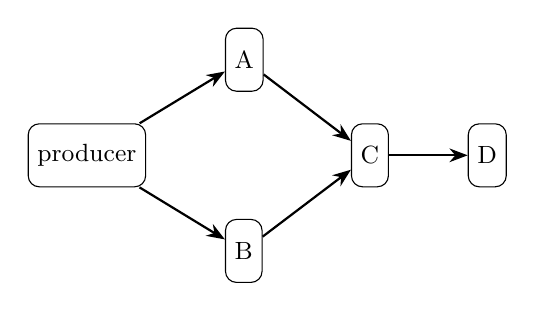
\begin{tikzpicture}[node distance=0.4cm and 1.0cm]
  \node[box] (p) {producer};
  \node[box, above right=of p] (a) {A};
  \node[box, below right=of p] (b) {B};
  \node[box, right=2.6cm of p] (c) {C};
  \node[box, right=of c] (d) {D};
  \draw[arrow] (p) -- (a);
  \draw[arrow] (p) -- (b);
  \draw[arrow] (a) -- (c);
  \draw[arrow] (b) -- (c);
  \draw[arrow] (c) -- (d);
\end{tikzpicture}
\end{center}
        So each edge numbers its offers with \code{seq}, which only
        increases. The two offers of frame 42 to D then get different
        \code{OfferId}s.
  \item Every message sent to an engine, every outcome, and every result
        event carries both ids.
\end{itemize}

\section{Flow control}
\label{sec:flow}

\subsection{End-to-end tokens}
\label{sec:tokens}

Each producer of a flow has a pool of $C$ tokens, owned by the client. If a
producer feeds several flows, each flow has its own pool, so the flows run
at independent rates. An input keeps its token along its whole path, on the
device and on the cloudlet. The token returns when the input \emph{first
completes}:
\begin{itemize}[nosep]
  \item \textbf{In series}, the input keeps its token through every engine of
        the chain. If an engine discards the input, the token returns right
        away. If the engine passes the input on, the token stays with it until
        a later engine completes it.
  \item \textbf{At a fan-out}, the paths race, and the token returns at the
        first completion on any of them. The producer therefore sends inputs as
        fast as the fastest path can process them, just as Gabriel does today
        with several engines.
\end{itemize}
The fastest path can change from one input to the next. Take a producer that
feeds both a local detector and a filter in front of a remote detector. For a
frame the filter discards, the filter's path is fastest. For a frame the
filter passes, the local detector's path usually is.

With sections (planned, \S\ref{sec:sections}), this pool becomes the first
of several. The input still keeps the producer's token along its whole path,
until its first completion anywhere, as above. In addition, at each fan-out
it takes a token from the pool of every branch it enters, and gives that one
back at its first completion in that branch. A branch with no token skips the
input before any work on it.

\paragraph{The producer's rate.} Each token carries one input at a time: an
input takes the token, and the token comes back when that input first
completes. Let $T$ be the time an input takes to first complete when nothing
is waiting. Then $C$ tokens allow up to $C$ inputs every $T$. But each engine
processes one input at a time, so the producer can never go faster than the
slowest engine on the path:
\[
  \text{rate} \approx \min\left(\frac{C}{T},\ \text{rate of the slowest
  engine on the path}\right)
\]
Extra tokens therefore help only when part of $T$ is spent outside engines,
mostly on the network: they keep the engine busy while other inputs are in
transit. For example, take a remote detector that needs 0.1~s per frame, with
a network round trip of 0.2~s, so $T = 0.3$~s:
\begin{itemize}[nosep]
  \item With $C = 1$, the producer sends about 3.3 frames/s, and the detector
        is idle two thirds of the time, waiting for the network.
  \item With $C = 3$, it sends 10 frames/s, and the detector is always busy.
  \item With $C = 5$, it still sends 10 frames/s. The two extra tokens are
        not used: the crossing to the detector has capacity 3, as sized in
        \S\ref{sec:edges}, and the admission rule below only admits an input
        that can be sent right away.
\end{itemize}

\paragraph{Choosing $C$.}\label{sec:choosing-c} This is the rule for one
count per producer. Sections (\S\ref{sec:sections}) would replace it with
tighter counts, measured at runtime. Tokens bound how many inputs
are in flight; they should never be what keeps an input fresh or stale. A
waiting input stays fresh only if a newer one can reach its pending slot and
replace it (``Freshness'' in \S\ref{sec:edges}), and a newer input needs a
token to get there. So $C$ must leave a token over when every place that can
hold an input holds one:
\[
  C \;\ge\; \text{engines} + \text{server edges} + 1,
\]
counting the engines on the producer's paths, one input in work each, and the
server edges leading to them, one pending input each. For one engine that is
3; for a chain of $k$ engines, $2k + 1$. The count is of places, not paths:
an engine that several branches reach counts once, and each of its incoming
edges counts, since each has a pending slot. At a fan-out this is more than
needed. An input holds its token only until its first path finishes, so
inputs left only on a slower branch hold none, and that branch is kept fresh
by its own edges. But which branch finishes first depends on service times
the compiler does not know, and extra tokens cost nothing in freshness, so
the compiler counts every place.

Why not count only the longest path? Because the inputs that hold tokens do
not have to lie on one path. An input skipped at a fan-out's fast engine has
not completed, so it still holds its token while it moves down the slow
branch. One input can be in the slow branch's last engine, another in its
pending slot, a third at the fast engine, and so on, until every place on
every branch holds a token. So only the count of places is sure to leave one
over. In a chain the two counts are the same. And the costs are lopsided: one
token too many costs a skipped copy, one too few can freeze a slot (398\,ms
at p99, below).

In a chain, a replaced input gives its token back at once: being skipped
in a pending slot ends its last open offer, so its ticket closes. (At a
fan-out it may still have an offer open on another branch, and then it keeps
its token, as above.) So in a chain the spare token is never used up. It
brings in a newer input, which replaces an older one, and the older one's
token becomes the spare. A pending slot behind an engine,
such as B's in P $\to$ A $\to$ B, is kept fresh by that engine's results,
whatever the token count. The spare token matters for the slots the client
feeds. In that chain, with A slower than the camera and B much slower, 4
tokens fill all four places, so the input waiting for A holds the last token
and waits for all of A's time. That makes B's inputs 60\,ms older at the
median. 5 tokens avoid this (\code{docs/evaluation.tex}).

A crossing to the remote server adds its
capacity, because inputs on the network hold tokens too. Fewer tokens fail in two ways, which
the token sweep in \code{docs/evaluation.tex} measured:
\begin{itemize}[nosep]
  \item \textbf{Fewer than the engines} lose pipelining: engines idle while
        others work. A chain of three equal engines gave a third of the
        results with one token as with three.
  \item \textbf{Exactly enough to fill the pending slots} freezes them. With
        2 tokens and one engine, the input in the pending slot holds the last
        token, so nothing can replace it, and it waits for the rest of the
        engine's time. With a heavy-tailed engine, the waiting Gabriel added
        was 398\,ms at p99, against 20\,ms with 3 tokens.
\end{itemize}
The bound is above the knee (\S\ref{sec:objective}): on one machine, the
knee is at most the number of engines on the path, and the rest covers the
pending slots and the spare. More tokens than the bound cost nothing in
freshness. Extra inputs are
skipped in the pending slots, and on one machine each costs a copy. They are
also not a way to send more over the network: a remote crossing admits only
what its capacity allows, and inputs beyond that wait, and are replaced, in
the client's pending slot. So the network is bounded by crossing capacities
(\S\ref{sec:edges}), and tokens by the whole flow. The compiler computes
this bound for each producer (\code{token\_bound} in
\code{client/compile.rs}), and uses it when the spec gives no count. A spec
may still give one; a count below the bound is used, with a warning.

\paragraph{Admission.} The client keeps only the newest input from each
producer, as its client thread does (\S\ref{sec:client-thread}). It admits that input into a flow
only when both of these hold:
\begin{itemize}[nosep]
  \item the producer's pool for the flow has a token, and
  \item at least one of the producer's outgoing edges can send the input
        right away.
\end{itemize}
The second condition stops the client from admitting inputs while every
engine they could go to is busy. Such inputs would only wait in pending
slots and replace each other there, so they would be admitted for nothing.
Worse, at a fan-out they can break alignment (\S\ref{sec:aligned}). Take a
producer feeding a fast engine F and a slow engine S, with several tokens:
\begin{enumerate}[nosep]
  \item F is busy with frame 4 and S with frame 1. A spare token admits
        frame 5, which waits in both pending slots.
  \item S finishes frame 1 and takes frame 5 from its slot.
  \item F is still busy. Another spare token admits frame 6, which replaces
        frame 5 in F's slot.
\end{enumerate}
S then processes frame 5, but F never does, so a fusion engine gets a slow
result for frame 5 with no fast result to match it. With the second condition,
an input is admitted only when an engine can take it right away. At a fan-out
that is normally when F has just become free, so F takes every admitted
input.

\paragraph{Consequences.}
\begin{itemize}[nosep]
  \item \textbf{The producer adapts to the whole path.} If the network or any
        engine on the fastest path slows down, tokens come back more slowly,
        and the producer sends fewer inputs. At most $C$ inputs per producer
        and flow are in flight at any time.
  \item \textbf{Early discard adapts to the scene.} Discarded frames return
        their tokens quickly, so the producer sends more frames. Frames that
        pass keep their tokens until the cloudlet replies, so the rate drops
        to what the cloudlet and the network can handle.
\end{itemize}

\subsection{Edges: capacity and the pending slot}
\label{sec:edges}

At a fan-out, the token returns when the fastest path completes. The producer
then admits the next input while slower branches are still busy, so inputs
arrive at a slow engine faster than it can process them. If every input were
sent to it, its queue would grow without limit. For example, with a fast
branch at 10 frames/s and a slow engine at 3 frames/s, the slow engine's queue
would grow by 7 frames every second. After 10~s, it would be processing frames
that are over 20~s old, and the gap would keep growing.

To prevent this, every input edge has a \emph{capacity} and a \emph{pending
slot}. An engine processes one input at a time, so the capacity does not let
it process more at once. Instead, it limits how many inputs from the edge can
be \emph{in flight}: the one being processed, plus any waiting in the
engine's queue or, for a crossing, still on the network. The pending slot
holds only the newest input that could not be sent yet. Older inputs are skipped.
The slow engine still processes only 3 frames/s, but each time it finishes, it
takes the newest frame. So the frames it works on stay about one processing
time old, instead of getting older and older; this is how slower engines skip
frames in Gabriel today. The process that owns the edge keeps this state for
it:

\begin{lstlisting}
struct EdgeState<T> {
    capacity: usize,
    in_flight: HashMap<OfferId, Sent<T>>,  // sent, not yet ended
    pending: Option<(OfferId, T)>,         // waiting, not yet sent
    actions: VecDeque<EdgeAction<T>>,      // what the owner must do next
    // ... plus the edge's id, a counter for offer ids, and the offer timeout
}
struct Sent<T> {
    offer: OfferId,
    deadline: Instant,   // the offer ends with TimedOut if still here then
    input: T,            // kept so the input can be forwarded after Pass
}
enum EdgeAction<T> {
    Send { offer: OfferId, input: T },
    Skipped { offer: OfferId, input: T },
    TimedOut { offer: OfferId, input: T },
}
\end{lstlisting}

The edge is generic over the input, \code{T}, because it only stores, clones,
and hands back inputs, so each process can store what suits it. The client's
edges hold only input ids, because the client keeps each input's data in its
ticket (\S\ref{sec:accounting}); a server's edges hold the data, or with zero
copy (\S\ref{sec:data}), a reference to it. Every action carries its input, so
the owner always knows which input a skipped or timed-out offer was for. The edge does no I/O and reads no clock. Its owner passes in the
current time, and collects the edge's \code{actions} (send this offer; report
that offer as skipped or timed out) and carries them out.

\begin{description}[nosep]
  \item[\code{in\_flight}] holds the offers that were sent to the engine and
        have not ended yet. An offer here may be travelling over the network,
        waiting in the engine's queue, or being processed. It stays here until
        it ends: when its \code{Result} arrives, when its deadline passes, or
        when its engine or connection is lost. Each entry keeps the offer's
        deadline, and the input itself, so that the process can forward the
        input if the engine reports \code{Pass} (\S\ref{sec:forwarding}).
  \item[\code{capacity}] is the most offers \code{in\_flight} may hold. The
        edge has \emph{spare capacity} while \code{in\_flight} holds fewer
        offers than that. A server's edges have no capacity: their pending
        offer is sent when the engine pulls it (``Engines with several
        incoming edges'' below).
  \item[\code{actions}] queues what the owner must do after each call:
        send an offer, or report one as \code{Skipped} or \code{TimedOut}.
  \item[\code{pending}] holds at most one offer that has \emph{not} been sent,
        because the edge had no spare capacity when the offer was made.
\end{description}

\paragraph{When an offer ends.} An offer is about a single edge: it ends when
the engine at the end of that edge is done with the input, not when the input
reaches the end of its path. It ends in exactly one of these ways:
\begin{itemize}[nosep]
  \item the engine reports its outcome (\code{Result}), whatever the outcome
        is;
  \item it is replaced in the pending slot before it was sent
        (\code{Skipped});
  \item its deadline passes, or its engine or connection is lost
        (\code{TimedOut} or \code{Disconnected}).
\end{itemize}
If the engine passes the input on, the offer still ends. Forwarding creates
\emph{new} offers on the engine's outgoing edges, each tracked by the process
that owns that edge, and each ending on its own. Three levels must not be
confused:
\begin{center}
\small
\begin{tabular}{@{}p{0.14\linewidth}p{0.5\linewidth}p{0.28\linewidth}@{}}
\toprule
What ends & When & Tracked by \\
\midrule
an offer      & the engine at the end of one edge is done with it
              & the process that owns the edge \\
a path        & an outcome forwards the input to no edge (completion)
              & the client, from \code{Result} events \\
an input      & all its offers have ended; its token returned at its first
                completion & the client's ticket \\
\bottomrule
\end{tabular}
\end{center}

\paragraph{Why the edge tracks its offers.} The process that owns an edge
keeps \code{in\_flight} because it is the one that decides what to send along
the edge, and needs four things to do it:
\begin{enumerate}[nosep]
  \item \textbf{Backpressure.} The number of offers in \code{in\_flight} is
        how many inputs the engine has from this edge, being processed or
        waiting. Comparing it with \code{capacity} decides whether a new
        offer is sent or goes to the pending slot.
  \item \textbf{Sending the pending offer at the right time.} When an offer
        leaves \code{in\_flight}, the engine has room again, so that is the
        moment to send the pending offer.
  \item \textbf{Deadlines.} An engine may hang, or an input may be lost.
        Checking the deadlines in \code{in\_flight} lets the process end such
        offers with \code{TimedOut}, free their capacity, and keep the
        guarantee that every offer ends with exactly one event
        (\S\ref{sec:events}).
  \item \textbf{Forwarding.} After a \code{Pass}, the process needs the
        input to offer it to the next edge. The \code{in\_flight} entry
        keeps it until the engine reports.
\end{enumerate}
None of this needs tokens, so servers can keep it for their own edges
without knowing about tokens. The client's tickets track the input as a
whole (\S\ref{sec:accounting}).

\paragraph{Offering an input.} When the client admits an input, or an engine
forwards one, the input is offered to each of the node's outgoing input
edges, with a new \code{OfferId} for each edge:
\begin{enumerate}[nosep]
  \item If the edge has spare capacity, the offer is sent and added to
        \code{in\_flight}.
  \item Otherwise, the offer replaces the one in the pending slot, and the
        replaced offer ends with \code{Skipped}. Nothing is queued.
\end{enumerate}
When a sent offer ends, it is removed from \code{in\_flight}, which frees
one unit of capacity, and the pending offer, if any, is sent and moves into
\code{in\_flight}. So a slower branch always gets the newest input when it becomes free,
just as a slower engine does today. An offer in a pending slot still holds
its input's token, so it counts against $C$.

\paragraph{One pending slot per edge.} An edge connects one node to one engine
in one flow, so an engine has one pending slot for each of its incoming edges.
Two cameras feeding the same detector use two edges, and so two slots. So
does one camera feeding the detector in two flows, or two earlier engines
feeding it in one flow. A single slot per engine would not work: a busy source
would keep replacing another source's waiting input, and that source could
starve. With one slot per edge, each source keeps its own newest input
waiting, and the engine's server takes inputs from the edges in turn (see
``Engines with several incoming edges'' below). This matches the
client, which keeps the newest input from each producer.

\paragraph{The queue at an engine.} Of the inputs in flight on a client's
edge, one may be processed, and the rest are on the network or wait at the
server, in the pending slot of their target edge, where a newer input
replaces an older one. The server gives each engine one input at a time, so
no queue forms in front of the engine itself. The pending slot is not a
queue: it holds at most one input that has not been sent, and a newer input
replaces it.

So backpressure works by \emph{dropping at the sender}. When an engine is
busy, its edge has no spare capacity, and newer inputs replace older ones in
the sender's pending slot. An input is never dropped after it was sent,
because that would waste the bandwidth used to send it. Inputs waiting at an
engine are processed oldest first.

\paragraph{Choosing capacities.} Capacity trades latency against throughput.
Each extra input waiting at an engine adds one processing time of latency,
but too few inputs in flight leave the engine idle.
\begin{itemize}[nosep]
  \item \textbf{Edges between engines on one server} have no capacity. Their
        engine pulls the next input only when it finishes the last one, so no
        input waits at the engine (``Engines with several incoming edges''
        below).
  \item \textbf{Crossings to the local server} have capacity 3. This is the
        smallest capacity that keeps the server's pending slots fresh
        (``Freshness'' below). There is no network delay to hide.
  \item \textbf{Crossings to the remote server} must hide the network round
        trip. With capacity 1, the remote engine sits idle for a whole round
        trip between inputs. The right capacity is the bandwidth-delay
        product of the path:
        \[
          \text{capacity} \approx \left\lceil
          \frac{\text{RTT} + \text{processing time}}{\text{processing time}}
          \right\rceil
        \]
        Then the next input arrives just as the engine becomes free. The
        inputs in flight are on the network, not waiting at the engine, and
        the queue stays close to empty. The token count must not play this
        role: a count tight enough to limit the link would freeze the
        server's pending slots (``Choosing $C$'' in \S\ref{sec:tokens}). A
        larger capacity does not increase throughput; it only
        makes the queue longer. Below 3, the remote engine may start on
        inputs one processing time old (``Freshness'' below); at 3 or more,
        the client sends inputs at the rate it admits them, and the server
        skips most of them. Which matters more depends on the link.
\end{itemize}
A crossing's capacity starts as a configured value. Later, the client can
adjust it from the round-trip and processing times it measures, much as TCP
adjusts its window. The capacity then follows a network or an engine that
slows down.

\paragraph{Optional age limit.} For some flows, a stale result is worse than
no result. Such a flow can give an edge a maximum waiting time. An input that
waits at the engine longer than that is dropped and ends with
\code{TimedOut}. This wastes the bandwidth used to send it, so it is off by
default.

\paragraph{Engines with several incoming edges.} An engine can receive inputs
on several edges: from one flow (fan-in), or from several flows or clients.
Its server's edges hold each input in their pending slots, and the engine
\emph{pulls} them:
\begin{itemize}[nosep]
  \item An engine has \emph{room} when no input delivered to it is without an
        outcome (\code{ENGINE\_DELIVERY\_LIMIT} is 1). The server counts this
        itself; the engine is never asked.
  \item While the engine has room, the server takes the next edge with a
        pending input, in turn (round-robin), sends that input, and delivers
        it into the engine's input service. Its deadline starts then.
  \item Until then the input stays in the edge's pending slot, where a newer
        input on the same edge replaces it, as on any edge. So the engine
        always gets each edge's newest input, however many edges feed it.
        Pending inputs have no deadline.
  \item A delivered input counts until its outcome arrives, even if its offer
        timed out before. A hung engine therefore gets no more inputs, and its
        input buffer never fills.
  \item What waits at the server is at most one input per edge. Adding an
        edge, a flow, or a client adds to the server's memory, not to the
        engine's buffer, which cannot grow at runtime.
\end{itemize}
Sending an input as soon as an edge has spare capacity would be wrong here:
with many edges, sent inputs would queue at the server behind each other,
older than the newer inputs that wait in the same edges' pending slots.

\paragraph{Freshness.} What matters is how old an input is when its engine
\emph{starts} on it. Waiting in front of a busy engine costs nothing, as long
as a newer input can replace the waiting one: when the engine becomes free,
it takes the newest input there is. Age is only added where an input is
\emph{committed} but not yet processed, because nothing can replace it there.
So the rule is: in front of a busy engine, every waiting place is
replaceable, and the only committed input is the one in work. Three places
could break the rule.
\begin{itemize}[nosep]
  \item \textbf{The engine's input buffer.} iceoryx2 cannot take back a sample
        it delivered. If the server delivered a second input ahead of time, as
        a ready input for when the engine finishes, the engine would start on
        it one processing time $T$ after it arrived, while a newer input waited
        at the server. In steady state, every slow engine would start on
        inputs $T$ old, and its results would come about $2T$ after their
        inputs. So the server delivers one input at a time. The cost is a
        short idle gap after each outcome: the outcome reaches the server, and
        the next input reaches the engine. On one machine these are two
        iceoryx2 hops, 46\,\textmu s at the median, against milliseconds of
        inference (\S\ref{sec:server-thread}). The server wakes on the
        engines' notifications, not on a timer, or the gap would grow to the
        timer's period.
  \item \textbf{The server's pending slot of a crossing target.} The client
        sends a crossing input only while the crossing has spare capacity, and
        an input sent on it stays in flight until the first of its targets ends
        it (\S\ref{sec:crossing}). A server edge holds at most one delivered
        and one pending input. So when all targets are busy, two crossing
        inputs can be in flight with no child ended. With capacity 2 the
        crossing is then full, the client stops sending, and the input in the
        server's pending slot is never replaced: the engine starts on it one
        processing time late. With capacity 3, the third input replaces the
        pending one at every target, which ends a child with \code{Skipped}
        and frees the crossing. So the server's pending slots keep getting
        the newest input. In general the capacity must be at least the
        delivery limit plus 2.
  \item \textbf{The producer's tokens.} They limit the same way: if every
        token is held by an input in work or in a pending slot, no newer
        input can come, and the pending input is never replaced. So the token
        count must leave one over (``Choosing $C$'' in \S\ref{sec:tokens}).
\end{itemize}
For example, take a camera P that feeds a fast engine F, and a chain
A $\to$ B $\to$ S whose last engine S is slow, all on the local server. P's
edges to F and A form one crossing, so each time F finishes, the crossing
frees and the newest input reaches both F's and A's pending slots. B and S
each start on the newest output of the engine before them. Inputs that S
later skips still cost compute at A and B; gating on downstream readiness
would save it (deferred, see the open questions).

\subsection{Crossings}
\label{sec:crossing}

Suppose a node has client-owned edges to several engines on the \emph{same}
server. The input should travel to that server only once. So these edges form
a single crossing, owned by the client, with one capacity and one pending
slot:
\begin{itemize}[nosep]
  \item The client offers the input to the crossing once, and sends it with
        the list of target engines.
  \item The server creates one offer per target engine on its own edges, each
        with its own pending slot. It reports these offers to the
        client in an \code{Accepted} event.
  \item The crossing's capacity is freed when the \emph{first} of these
        offers ends, however it ends: with a \code{Result}, or with
        \code{Skipped} when a newer input replaced it at the server. Slower targets take the input from the server when they
        become free, unless a newer input has replaced it. This is today's
        Gabriel server rule. It also means the crossing never sends an input
        that no target will process.
  \item The crossing's timeout covers the whole wait: the trip to the server
        and the first target's work. If no target finishes in time, the
        crossing times out and frees its capacity. Its children stay open in
        the ticket, and their later events are applied as usual, but they do
        not free the crossing again.
\end{itemize}
The client remembers which crossing each child came from, from
\code{Accepted} until the first child ends.
The common case, an ordinary uplink, is a crossing with one target. Every
client-owned edge that ends at a server's engine is a crossing, including an
edge from a producer to a local engine, so a server receives inputs from the
client in only one way. On its ordered stream to the client, the server
reports one \code{Accepted} event that lists every target's offer; it names
no engine, because it covers them all. On the
event services of the engines (\S\ref{sec:subscribe}), it publishes one
\code{Accepted} on each target engine's service, listing only that engine's
offer, so that each engine's events stay on its own service. An input
goes over the network only when it holds a token and its crossing has spare
capacity. So the inputs travelling to or waiting at the remote server never
exceed the crossing's capacity.

While the client is not connected to a server, every crossing to that server
has no spare capacity. Offers to it wait in the pending slot and are replaced
by newer ones, so nothing piles up during a disconnection, and an input whose
only path leads to that server is not admitted at all. The offer pending when
the connection is lost is skipped, so that nothing old is sent once the
server is back.

When the client skips an offer in a crossing's pending slot, the target
engines' subscribers must learn it too, e.g.\ fusion waiting for a local
result. For a local engine, the local server is the only publisher of its
event service. So the client sends the server a skip notice next to its
inputs, and the server publishes \code{Skipped} on each target engine's event
service. The notice does not go to the client's own event stream: the client
already knows.

\subsection{Alignment at a fan-out}
\label{sec:aligned}

Fusion needs results from two branches for the \emph{same} input. The rules
above already provide this, without any extra mechanism. Take a producer that
feeds a fast engine and a slow engine:
\begin{enumerate}[nosep]
  \item The token returns when the fast engine finishes. That is when the
        next input is admitted, and the fast engine is free to take it. So
        every admitted input reaches the fast engine.
  \item The slow engine takes the newest admitted input from its pending slot
        whenever it becomes free.
  \item So every input the slow engine processes is also processed by the
        fast engine.
\end{enumerate}
This is today's server rule, with one difference. If the slow engine becomes
free after the fast engine finished an input, but before the next input is
admitted, it takes the input the fast engine just finished. Today it would
wait for a new input instead. The input it takes already has a fast result,
which suits fusion, but it may be up to one fast-engine processing time older.

As with today's server, alignment fails in two cases:
\begin{itemize}[nosep]
  \item \textbf{The faster branch changes}, e.g.\ the cloudlet sometimes
        finishes first. An input admitted for the branch that was faster can
        then be replaced in the other branch's pending slot, and gets only
        one result.
  \item \textbf{The branches start at different nodes}, e.g.\ producer $\to$
        A $\to$ X and producer $\to$ B $\to$ Y. A and B skip inputs
        independently, so X and Y can see different inputs.
\end{itemize}
In both cases, the result events tell the fusion engine that a result will not
come (\S\ref{sec:events}), so it uses the one it has.

\subsection{Are tokens the right tool?}
\label{sec:alternatives}

\paragraph{What tokens were for.} In the original Gabriel, a producer sends
to one engine on the cloudlet. The path is one link and one engine, so a
window on the path is a window on that engine. Tokens were exactly the right
limit there.

\paragraph{What they do in a DAG.} Here the path has many places where an
input can wait, and one token count covers all of them. The token sweep
(\code{docs/evaluation.tex}) shows three regimes:
\begin{itemize}[nosep]
  \item \textbf{Below the knee}, tokens cost throughput. A chain of three
        equal engines had a third of the results with one token as with
        three, and its AoI was 97\,ms instead of 77\,ms.
  \item \textbf{Exactly as many as the places that hold inputs}, tokens
        freeze a pending slot (``Choosing $C$'' in \S\ref{sec:tokens}). One
        heavy-tailed engine got 3\% more use with 2 tokens than with 1, but
        its average AoI rose from 105\,ms to 147\,ms.
  \item \textbf{Above that}, tokens do nothing. With 7 tokens on the
        three-engine chain, 0.9 inputs were in flight on average, and every
        measure was the same as with 3 or 10.
\end{itemize}
So in a DAG, tokens either get in the way or are not used. The work is done
per hop: newest-wins pending slots, engines that take one input at a time,
and crossing capacities. Tokens keep two smaller jobs: a hard cap on how many
of a producer's inputs are in the system, which bounds the client's memory,
and the tickets that let the client tell the app what happened to each input
(\S\ref{sec:accounting}). Tickets do not need the cap to be tight.

\paragraph{What a token means.} A token stands for an input that is still
alive and has not given a result on any path. It comes back at the input's
first completion, or when the input dies: its last offer ends without any
path completing. An input replaced at one engine of a fan-out keeps its token
while it is still alive on another branch, for two reasons:
\begin{itemize}[nosep]
  \item \textbf{The input is not done.} It still holds a place on the other
        branch. Returning its token would let more inputs in than the count
        says.
  \item \textbf{A skip signals too much supply, not free capacity.} A skip
        means a newer input arrived; a completion means work finished.
        Returning tokens on skips would admit more inputs exactly when there
        are too many.
\end{itemize}
The rule only matters when tokens are scarce. With $C$ set by ``Choosing
$C$'', there is always a spare token, and the rule decides nothing. With
sections (\S\ref{sec:sections}), counts are tight, and it matters: an input
that the fast branch skipped, but that is alive on a slow branch, holds the producer's
token until the slow branch completes it (see the open questions).

\paragraph{Two goals: freshness or compute.} A low token count is tempting
as a way to save compute: fewer inputs enter, so fewer are processed and
then skipped. In a chain whose last engine is much slower than the rest, it
works. With a camera at 30 frames a second, A at 50\,ms, and B at 500\,ms
(\code{docs/evaluation.tex}):
\begin{itemize}[nosep]
  \item \textbf{1 token:} A works only on inputs B will take. A does a
        tenth of the work, B loses 7.5\% of its throughput to waiting for A,
        and B's mean AoI is the same as with 5 tokens. A's own results are
        older: 340\,ms of AoI instead of 92\,ms.
  \item \textbf{2 tokens:} B's pending slot freezes, and B starts on inputs
        525\,ms old. The worst count.
  \item \textbf{3 to 5 tokens:} A works at full rate, and B skips 90\% of
        A's results.
\end{itemize}
But a token count is the wrong control for compute, for two reasons:
\begin{itemize}[nosep]
  \item \textbf{It depends on the shape.} In a chain of equal engines, one
        token gives a third of the throughput. Only a chain with one slow
        engine gets it nearly free.
  \item \textbf{It cannot act on one branch.} At a fan-out, the token comes
        back when the fastest branch completes, so a slow branch skips as
        much with one token as with ten (82\% in the fan-out sweep). One pool
        per producer cannot say ``keep F at full rate, but feed B's branch
        only as fast as B uses it''.
\end{itemize}
What fits is one pool per section, sized by the section's own shape
(\S\ref{sec:sections}). A branch's pool feeds that branch only as fast as it
completes inputs, while F keeps the pace of its fastest branch. So a chain
on a slow branch, such as A $\to$ B, gets the 1-token behavior where it
helps, and a chain of equal engines gets the 3 tokens it needs. The cost is
an idle gap: once B finishes, it waits for A, which was 7.5\% of B's
throughput above. Predictive pull could close it later, by admitting an
input about one upstream processing time before B is expected to finish;
the count would then be a time rather than a number. An earlier plan had
two modes per edge, fresh and gated, set in the spec. Sections replace it:
they gate only where the measured counts say work would be skipped.

\paragraph{The alternatives.} These are the approaches that can limit
waiting, each with the cost it pays:
\begin{description}[style=nextline, leftmargin=1.5em, nosep]
  \item[Per-hop limits (today, under the tokens)] Each hop limits what it
        holds: one input in work per engine, one pending input per edge, and
        a capacity per crossing. Networks call this credit-based flow control
        (as in ATM and InfiniBand). Waiting is limited where it happens, and
        throughput is kept as long as each limit is above that hop's own
        knee. On the device, this is enough.
  \item[Adaptive crossing capacity] A remote crossing's capacity is the
        control that matters over the network. Instead of a fixed number, the
        client can adjust it as TCP Vegas and BBR adjust their windows: grow
        it while the remote engine sits idle between inputs, and shrink it
        while inputs wait at its edge. Both signals are already measured: the
        wait from each event's \code{offered\_at}, and the idle time from the
        gap between a result and the next \code{Sent}.
  \item[Pacing] The client sends at the rate the remote engine finishes
        inputs, instead of in bursts when capacity frees. This smooths
        arrivals, which shortens waits; it works together with an adaptive
        capacity.
  \item[Predictive pull] The server asks for the next input one round trip
        before it expects its engine to finish. If the guess is right, there
        is no waiting, no idle time, and no waste. If the engine finishes
        early, it idles; if late, the input waits. It needs a request message
        on the crossing and a prediction of the service time, which a heavy
        tail makes hard. A safety margin, tuned from the measured idle time
        and wait, sets the balance.
  \item[Age limit (optional today)] Drop an input that waited too long. It
        caps the worst waiting, but wastes what was already sent, and it does
        not lower the average.
  \item[Gating on downstream readiness (planned, as sections)] An
        upstream engine starts an input only if its section's pool has a
        token, so its output will be used (\S\ref{sec:sections}). It saves
        upstream compute, at the cost of downstream idle time (``Two goals''
        above). On a device whose engines share a GPU, it may lower the AoI
        overall. With predictive pull, it may keep both.
  \item[On-demand producers] Capture a frame when the path is ready for it,
        so that no frame waits for a token. This removes the waiting before
        admission, which for a camera is up to one frame period. Producers
        that cannot capture on demand keep only their newest frame.
\end{description}

\paragraph{Conclusion.}
\begin{enumerate}[nosep]
  \item \textbf{Tokens stay.} Today the compiler sets one count $C$
        per producer by the rule in ``Choosing $C$'', so tokens never decide
        which input is fresh. A spec may still give a count, as a cap.
        Tickets and the accounting built on them do not change.
  \item \textbf{One count for the flow is not the way to save compute.} A
        low count helps only in a chain with one slow engine, freezes slots
        at some counts, and cannot act on one branch of a fan-out. One pool
        per section can, with inputs waiting in order and each count kept at
        its knee while the flow runs (\S\ref{sec:sections}). It needs
        estimates that err low, and code, so it pays off where skipped work
        costs something.
  \item \textbf{On the device, the per-hop limits are the control, and
        sections are the next step to measure:} first on the bench's chain
        and fan-out against the single count, then with engines that share
        a GPU, then with predictive pull. The measurements decide whether
        sections become the default or an option per flow.
  \item \textbf{Over the network, the crossing capacity is the control.}
        With the remote server, start with an adaptive capacity, since it
        needs only signals that exist; then compare it with predictive pull
        on emulated links.
  \item \textbf{Every comparison uses the AoI}, with waiting, idle time, and
        waste to explain it.
\end{enumerate}

\subsection{Sections (planned)}
\label{sec:sections}

This is the planned replacement for the single token count of ``Choosing
$C$''. None of it is built yet. The idea is the original Gabriel, applied
again at every fan-out: each part of the flow between fan-outs gets its own
pool of tokens, its inputs wait in order instead of being skipped, and each
pool keeps its count at the knee (\S\ref{sec:objective}), measured while the
flow runs.

\paragraph{Sections.} A section starts at a producer, or at an edge that
leaves a fan-out (an engine with two or more outgoing edges). It runs along
the chain that follows, up to the next fan-out or the end of the path. Each
section has its own pool. Take P $\to$ F $\to$ \{C, A $\to$ B\}:
\begin{itemize}[nosep]
  \item \textbf{R} covers P $\to$ F,
  \item \textbf{c} covers the branch C, and
  \item \textbf{ab} covers the branch A $\to$ B.
\end{itemize}
To R, everything below F is one \emph{box}. R does not see inside it; it
only sees when the box returns its first result for an input.

\paragraph{When tokens are taken and returned.}
\begin{itemize}[nosep]
  \item \textbf{An input enters a section only with a token from its pool.}
        At the producer, this is admission, as today.
  \item \textbf{The token returns at the input's first completion in the
        section}, or when the input dies there. This is the ticket rule of
        \S\ref{sec:tokens}, applied to a section instead of the whole flow.
  \item \textbf{The rule is recursive.} The first completion in a box is the
        first among its branches, and a branch's first completion is the
        first in its own boxes. So R's token returns when the fastest branch
        of F's box completes, and a later completion on another branch
        returns only that branch's token. R's rule is the same as today's:
        the first completion anywhere below the producer.
\end{itemize}

\paragraph{Waiting in order, not skipping.} Inside a section, an input that
finds its next engine busy waits in a queue on the edge, and the engine takes
the oldest one first. No input is skipped after work was spent on it. The
queue needs no limit of its own: a section with $N$ tokens holds at most $N$
of its inputs, so at most $N - 1$ wait anywhere in it. (When $N$ drops, a
queue can hold more for a moment, since nothing is recalled.) Inputs are
dropped in only two places, and neither wastes work:
\begin{itemize}[nosep]
  \item \textbf{At the producer,} which keeps only its newest input until a
        token is free, as today. Nothing was computed on the inputs it
        replaces.
  \item \textbf{At a branch's entry.} F's result enters a branch only if the
        branch's pool has a token, and a newer result replaces one waiting
        there. A branch may drop a result only if another branch took it, so
        F's work is never lost: a result that no branch has taken yet waits
        at the fan-out until one has a token.
\end{itemize}
This is what makes a section a closed queueing network in the usual sense,
which the count below assumes. It also helps alignment
(\S\ref{sec:aligned}): a branch processes every input it took.

\paragraph{The count.} The knee of a closed network follows from bound
analysis (Lazowska, Zahorjan, Graham, and Sevcik, 1984). It is built from
parts that can each be measured:
\[
  N^* = \frac{D + Z}{\max(D_{\max},\ I)}, \qquad
  N = \max\left(1,\ \lfloor N^* + \epsilon \rfloor\right)
\]
\begin{itemize}[nosep]
  \item $D$ is the \emph{service demand} per input: the sum over the
        section's engines of $V_k S_k$. $S_k$ is engine $k$'s service time,
        and $V_k$ its \emph{visit ratio}: the share of the section's inputs
        that reach it. A filter that passes a third of its inputs gives the
        engine after it $V = 1/3$.
  \item $Z$ is the pure delay per input: the network round trips on the
        section's crossings, each weighted by its visit ratio.
  \item $D_{\max}$ is the largest $V_k S_k$: the bottleneck's demand.
  \item $I$ is the producer's interval between inputs, for the producer's
        own section. When the producer is slower than every engine, it sets
        the pace, and fewer tokens are needed.
  \item \textbf{A box counts as one stage.} Its time, which goes into
        $D + Z$, is that of its branch that completes first. Its demand,
        which competes for $D_{\max}$, is the smallest $D_{\max}$ among its
        branches, since the branch with the highest rate sets the pace.
  \item $\epsilon$ is \code{ROUNDING\_TOLERANCE}: a knee just below a whole
        number counts as that number. Three equal engines give $N^* = 3$
        exactly, and measurement noise puts it at 2.99; a plain floor would
        give 2 tokens and lose a third of the throughput.
\end{itemize}
The count is rounded down because with queues in order, each token above the
knee adds one bottleneck time of waiting to every input: in the chain with a
slow end, every token above 1 adds 500\,ms to B's AoI. Rounding down leaves a
stage idle instead, but keeps at least $\lfloor N^*\rfloor / N^* \ge 1/2$ of
the throughput. The simulation in \code{docs/evaluation.tex} confirms that
this floor is the best count with queues in order, in all four chains
measured.

Three other ways to get the count do not work:
\begin{itemize}[nosep]
  \item \textbf{The pool's own rate and time.} With $N$ tokens, the measured
        rate is $N/W$, so Little's law always gives $N$ back, and the count
        could never grow.
  \item \textbf{The shortest time from taking a token to its return}, over
        the bottleneck's time. It works when every input takes the same
        path, but not with early discard: a filter that discards in 5\,ms
        makes the shortest time 5\,ms, and the count 1, while the inputs it
        passes spend 300\,ms on a remote detector and need 3.
  \item \textbf{Mean value analysis} (Reiser and Lavenberg, 1980), which
        predicts the throughput and delay for every $N$. Its approximation
        for service times that are not exponential fails for engines with
        nearly constant times: on three equal engines it predicted 33
        results a second at 3 tokens, against 49 measured, and so chose 2.
\end{itemize}

\paragraph{Measuring.} The client measures every part from what it already
receives, with no new messages:
\begin{itemize}[nosep]
  \item \textbf{$S_k$:} the time from an engine's \code{Sent} event to its
        \code{Result}. Both are stamped by the engine's server, so the
        offset between clocks cancels. Each new sample moves a smoothed
        value by a fixed share, \code{SERVICE\_TIME\_GAIN} (1/8, as TCP
        smooths its round trip in RFC 6298). Timed-out offers are not
        samples.
  \item \textbf{$V_k$:} from the share of results each engine forwards
        (\code{Pass} or \code{Emit}, against \code{Stop}), smoothed the same
        way, multiplied along the chain. Not from how many inputs reached
        each engine: with today's skips, B in the chain with a slow end sees
        a tenth of A's results, which would make it look ten times cheaper
        than it is.
  \item \textbf{$Z$:} for each crossing, the round trip that the QUIC
        connection already measures (quinn reports it), times the
        crossing's visit ratio.
  \item \textbf{$I$:} the mean gap between the producer's inputs, which the
        client sees as they are published.
\end{itemize}

\paragraph{Updating.}
\begin{itemize}[nosep]
  \item \textbf{At the start,} each pool has 1 token, until each engine of
        its section has \code{MIN\_SAMPLES} samples. One token is always a
        safe count: nothing waits.
  \item \textbf{After each returned token,} the client computes $N^*$
        again. Sections are small, so this is cheap.
  \item \textbf{Hysteresis} stops the count flapping near a boundary. The
        count rises to a new value only once $N^* + \epsilon$ is past it by
        $H$, and falls only once $N^* + \epsilon$ is below the current count
        by $H$, where $H$ is \code{COUNT\_HYSTERESIS}.
  \item \textbf{Raising} the count adds tokens to the pool at once.
        \textbf{Lowering} it recalls no input: returned tokens are dropped
        until fewer than $N$ are in use. The pool's invariant
        (\S\ref{sec:accounting}) then reads: available plus held tokens
        equal $N$, except while more than $N$ are held.
  \item \textbf{A count in the spec} becomes a cap on $N$.
  \item \textbf{Pools on a server} (below) get their counts from the client
        with a control call when they change. Hysteresis keeps such calls
        rare.
\end{itemize}
A shadow run of this estimator on recorded bench runs
(\code{docs/evaluation.tex}) gave the same estimates whatever token count the
run used, and changed the count at most once per run.

\paragraph{Examples.}
\begin{itemize}[nosep]
  \item \textbf{A chain with a slow end}, A at 50\,ms and B at 500\,ms:
        $N^* = 550/500 = 1.1$, so $N = 1$. A does a tenth of the work, B
        loses 7.5\% of its throughput, and B's AoI is the same as the best
        today.
  \item \textbf{Three equal engines in a chain}: $N = 3$, the knee the token
        sweep found.
  \item \textbf{The bench's chain}: a camera every 33\,ms, a 2\,ms filter
        that passes half, a 44\,ms detector, and a 5\,ms tracker. $D = 2 +
        22 + 2.5 = 26.5$\,ms, and the camera's 33\,ms is slower than the
        detector's demand of 22\,ms, so $N^* = 0.8$ and $N = 1$.
  \item \textbf{A remote detector} at 0.1\,s per frame, with a round trip of
        0.2\,s: $N^* = (0.1 + 0.2)/0.1 = 3$, as in ``The producer's rate''.
        As with the original Gabriel's tokens, the count covers the round
        trip.
  \item \textbf{Early discard}: a filter at 5\,ms that passes a third of its
        inputs to that remote detector. $D = 5 + 100/3 = 38$\,ms, $Z =
        200/3 = 67$\,ms, and $D_{\max} = 33$\,ms, so $N^* = 3.2$ and $N =
        3$. Little's law agrees: the detector takes 10 inputs a second, so
        the filter takes 30, and an input spends 105\,ms on average.
  \item \textbf{A fan-out}, with F at 50\,ms, C at 100\,ms, A at 50\,ms,
        and B at 500\,ms. Branch c has $N^* = 1$, and branch ab has $N^* =
        1.1$, so both get 1 token. For R, the box's time is C's 100\,ms, and
        its demand is $\min(100, 500) = 100$\,ms, so $N^* = (50 + 100)/100 =
        1.5$, and $N = 1$. F works at the pace of C. A takes one of F's
        results only after B finishes its last one, so A does no work that B
        skips. If C slows down past A $\to$ B, the estimates follow, and no
        part of the rule names the fast branch. Not simulated or measured
        yet.
\end{itemize}

\paragraph{Is it better than one count?} Not in every case. In simulation,
validated against the token sweeps (\code{docs/evaluation.tex}), sections
with their counts gave:
\begin{itemize}[nosep]
  \item \textbf{the same AoI as the best single count} in three of four
        chains: one heavy-tailed engine, three equal engines, and the chain
        with a slow end. In the last, they saved the 45\% of engine time
        that went to work B later skipped.
  \item \textbf{a 6\% higher AoI} in the bench's chain, whose filter passes
        inputs at random and whose detector has a heavy tail. With skips, an
        extra input in flight can be replaced by a fresher one when it would
        wait; in order, it waits.
\end{itemize}
They also cost:
\begin{itemize}[nosep]
  \item \textbf{A count that must not be too high.} With skips, tokens
        above the knee cost nothing (``Choosing $C$''). In order, each one
        adds a bottleneck time of waiting. So the estimates must err low,
        and an engine shared with other flows, or a remote engine whose
        round trip changes, is a risk. The single count needs no estimate.
  \item \textbf{Throughput.} Rounding down gives up to half of it, and an
        engine in the middle of a chain produces fewer results: in the chain
        with a slow end, A's own AoI went from 92\,ms to 340\,ms. That
        matters when the app reads A's results.
  \item \textbf{Code:} the estimates, the recount, tickets per section,
        queues on edges, pools on servers, and a control call to set their
        counts.
\end{itemize}
So sections pay off where skipped work costs something: engines that share
a GPU, or a device on a battery. Where every engine has its own hardware,
the single count gives the same or fresher results with less machinery.
Whether sections become the default, or an option per flow, is for the
measurements on fan-outs and shared engines to decide (``Conclusion''
above).

\paragraph{What stays.} Tickets, events, the engines' pull, and the second
condition of admission all stay. The pending slot becomes a queue inside a
section, and stays a newest-wins slot at a section's entry. A crossing keeps
its capacity as the limit on the link; a section's count, which covers the
round trip, is a natural starting value for it.

\paragraph{Where the pools live.} R stays at the client. A branch's pool
lives in the process that owns the branch's first edge: the client, for a
fan-out at a producer, or a server, for a fan-out at one of its engines. The
client computes every count. A server's pool sees completions only on that
server, so the first version gates only branches that stay on one server. A
branch that leaves it, to the client or over a crossing, stays ungated, as
today, and is limited by its crossing capacity.

\section{Moving inputs}
\label{sec:moving}

\subsection{Forwarding}
\label{sec:forwarding}

An engine decides \emph{what} to forward, never \emph{where}. Its outgoing
edges belong to the flow, so the same engine can be the last engine in one
flow and sit in the middle of another. The engine only reports a verdict. The
process that owns the next edge sends the input on, from a copy it kept:
\begin{itemize}[nosep]
  \item A server keeps every input it sent to one of its engines in the
        edge's \code{in\_flight} entry, until the engine reports
        (\S\ref{sec:edges}).
  \item The client keeps every input it admitted until the input is done,
        i.e.\ until its ticket closes. The edge's \code{in\_flight} entry is
        not enough for the client: in a cascade such as producer $\to$ A
        (local) $\to$ B (local) $\to$ uplink, A passes the frame to B over the
        local server's edge, and when B passes it on, the client must send the
        frame over the uplink, long after its own offer to A has ended.
\end{itemize}
Memory use is therefore limited by the number of inputs in flight.

\paragraph{Next engine on the same server}, e.g.\ remote detector $\to$
remote tracker:
\begin{enumerate}[nosep]
  \item The server keeps the input it received, from the client or from an
        earlier engine. It publishes the input on the detector's iceoryx2
        input service, and the detector reads it without a copy.
  \item The detector calls \code{gabriel\_engine\_pass}. The library publishes
        a \code{Pass} outcome on the detector's outcome service, and releases
        the input sample.
  \item The server offers its kept copy of the input to the edge from the
        detector to the tracker. If the tracker is free, the server copies the
        input into a sample of the tracker's input service and publishes it.
        Otherwise, the input waits in the edge's pending slot.
  \item The server reports a \code{Result} event with \code{Pass} to the
        client, listing the new offer as a child.
\end{enumerate}

\paragraph{Next engine across a crossing}, e.g.\ local filter $\to$ remote
detector:
\begin{enumerate}[nosep]
  \item The client admitted the frame and keeps it until the input is done.
        It sent a
        copy to the local server, which published it to the filter.
  \item The filter calls \code{gabriel\_engine\_pass}. The filter's outgoing
        edge is a crossing owned by the client, so the local server creates no
        offer. It reports a \code{Result} event with \code{Pass} and no
        children.
  \item The client offers the frame it already holds to the crossing. If the
        crossing has spare capacity, the client sends the frame to the remote
        server on a new QUIC stream.
  \item The remote server keeps the frame, creates the offer to the detector,
        reports that offer in an \code{Accepted} event, and publishes the
        frame to the detector, as in the first case.
\end{enumerate}
The filter only returns a verdict; the frame never travels back from it.

\paragraph{\code{Emit}} works the same way, except that the forwarded input is
new. The engine loans one output buffer and fills it, and the library
publishes it with the outcome. The server offers that new input instead of the
original one. Gabriel does not look inside it. If the engine produces several
tiles, it lays them out in the buffer itself, in a layout that its payload
type defines, and the next engine reads them the same way. The tiles travel as
\emph{one} input, so they are offered, sent, and skipped together. This
matters for tiles: tiles are parts of one frame, not newer versions of each
other, so one tile must not replace another in a pending slot.

\subsection{Copies}
\label{sec:data}
\label{sec:copies}

In iceoryx2, a received sample lives in the \emph{publisher's} shared memory.
A subscriber can read it and hold on to it for a while, but cannot republish it
through its own publisher, and a publisher cannot keep a sample after sending
it. So each time an input moves on to another process or engine, it is copied
into a new sample. In the first version, the input is copied at these points:

\begin{center}
\small
\begin{tabular}{@{}p{0.34\linewidth}p{0.6\linewidth}@{}}
\toprule
Where & What happens \\
\midrule
Producer $\to$ client
  & The client copies the frame out of the producer's sample into its own
    reference-counted buffer, once per frame, however many flows the frame
    enters. Each flow's ticket holds a handle to that buffer until the input
    is done. This releases the producer's sample right away. \\
Client $\to$ local server
  & The client copies the frame into a sample of its own service for the local
    server. \\
Local server $\to$ local engine
  & The server copies the frame out of the sample it received into its own
    reference-counted buffer, which it keeps while the input is in flight.
    It copies the frame from there into a sample of the engine's input
    service, once per engine it sends the frame to, including after
    \code{Pass}. Holding the received sample instead would save the first
    copy. \\
Client $\to$ remote server
  & quinn copies the frame into its send buffers, and the network carries
    it. \\
Remote server $\to$ remote engine
  & quinn assembles the received bytes into one buffer. The server copies
    them into its own reference-counted buffer, which it keeps while the
    input is in flight, and copies the frame from there into the engine's
    input sample, once per engine. Taking over quinn's buffer instead would
    save the first copy. \\
Engine $\to$ server after \code{Emit}
  & The engine writes the new input into a loaned outcome sample. The server
    copies it out into its own reference-counted buffer, and then treats it
    like any input it received. Keeping the outcome sample instead would avoid
    this copy, but each held sample takes a place in the engine's small outcome
    buffer, possibly for a long time. \\
\bottomrule
\end{tabular}
\end{center}

Every other step shares the copy it already has: the client's kept input, the
pending slots, and the \code{in\_flight} entries all hold an \code{Arc} or a
held sample, not a new copy. So a frame that goes from the producer through
one local engine and one remote engine is copied seven times: out of the
producer's sample, to the local server, out of the local server's sample,
into the local engine's input, onto the network, out of quinn's buffer, and
into the remote engine's input. Results are small, and are copied freely.

\paragraph{Zero copy on one machine.} iceoryx2 can deliver one published
sample to \emph{every} subscriber without copying it. Local engines can
therefore share inputs without copies, if the data is kept apart from the
routing messages:
\begin{enumerate}[nosep]
  \item \textbf{Data stays where it was first written.} A frame stays in its
        producer's input service. The input an engine emits stays in that
        engine's output service.
  \item \textbf{Readers subscribe to the data directly.} The client and every
        local engine of a flow subscribe to the services their inputs can come
        from. Each frame then reaches all of them for the cost of a pointer.
  \item \textbf{Routing messages point to the data.} Instead of sending the
        data, a server tells an engine ``process input $i$, which is at
        (service, sequence number, part)''. On \code{Pass}, the server sends
        the next engine the same reference; that engine already has the data
        in shared memory.
  \item \textbf{The engine's library matches references to samples.} It
        keeps the samples it has been told to process, or may soon be told
        to, and releases all other samples immediately. The engine still
        calls \code{poll\_input} and gets a pointer to the input, so the
        engine ABI does not change.
\end{enumerate}
A chain or fan-out of local engines then copies no frames. The only copy left
on the device is the one made when a frame is sent over the network. The
remote server writes each frame it receives once into a service of its own,
and its engines share it the same way.

\paragraph{Costs of zero copy.}
\begin{itemize}[nosep]
  \item \textbf{Held samples use up the producer's memory.} An input's sample
        stays held while the input is in flight. When every slot of the
        producer's service is held, \code{new\_input} fails. Tokens bound
        this: at most $C$ inputs per flow are in flight. So the producer's
        service is sized from the token counts of its flows, e.g.\ with
        \code{subscriber\_max\_borrowed\_samples} at least $C + 1$, and with
        \code{max\_subscribers} large enough for the client and the engines.
        When \code{new\_input} fails, the producer drops that frame, which is
        what Gabriel does anyway.
  \item \textbf{A reference and its sample can arrive in either order.} The
        library holds a reference until its sample arrives, and keeps recent
        samples for a short time in case a reference follows.
  \item \textbf{Every subscribing engine receives every frame.} This costs
        only a pointer, but each engine's subscriber buffer must be large
        enough to keep a frame it is about to be told to process.
  \item \textbf{More services, and less isolation.} Every engine of a flow can
        read every frame of its producers. This is acceptable on one device.
\end{itemize}

\paragraph{When it matters.} A raw 4K RGB frame is about 25~MB. An embedded
board has about 5--10~GB/s of memory bandwidth, so each copy takes about
2.5--5~ms. Several copies per frame at 30 frames/s use a large share of a CPU
core, and compete with the accelerator for memory bandwidth. A 1~MB JPEG frame
copies in about 0.1--0.2~ms, which is negligible.

\paragraph{Measured.} On a desktop (Intel Core Ultra 7 265K), a raw frame on
the local path is copied four times by Gabriel: twice in the app's process
(by the client) and twice by the server. The server's two copies cost 0.30,
0.73, and 2.5~ms of CPU per frame at 720p, 1080p, and 4K, about 18~GB/s. With
the app's own copy into the producer's sample, the copies are most of the
6.2~ms round trip of a 4K frame to an engine that answers at once
(``Comparison with the original Gabriel'' in \code{docs/evaluation.tex}).
Two ways to save them:
\begin{enumerate}[nosep]
  \item \textbf{Hold received samples instead of copying them into
        reference-counted buffers.} This saves the copy out of the producer's
        sample and the copy out of the server's, half of them, with no change
        in behavior. Samples cannot move between threads, so the client still
        copies an input that goes to a remote server, which costs a copy
        anyway. The number of samples a subscriber may hold must cover the
        inputs pending and in flight.
  \item \textbf{Zero copy on one machine}, as above, which saves all four.
\end{enumerate}

\paragraph{Plan.} Start with copies, which are simpler and let us measure the
cost. But make routing messages point to their data from the start
(\S\ref{sec:wire}). Switching to zero copy later then only changes the
transport, not tokens, events, or the engine ABI.

\section{Results}
\label{sec:results}

\subsection{Outcomes}

Engines report one outcome per input to their own server, over iceoryx2:
\begin{lstlisting}
struct Outcome {
    offer: OfferId,
    input: InputId,
    node: String,              // engine that produced it
    result: Option<Vec<u8>>,
    forward: Forward,          // Pass | Emit(output: Vec<u8>) | Stop
}
\end{lstlisting}
A discard is \code{Stop} with no result. An engine can pass an input on and
also report a result, e.g.\ a filter whose detections are used for
speculative action. The server applies the outcome to the edges it owns, and
reports it to the client as a \code{Result} event. The client then applies it
to the edges the client owns, such as an uplink after a local filter's
\code{Pass} (\S\ref{sec:forwarding}). The records and services that carry
outcomes and events on one machine are in \S\ref{sec:services}.

\subsection{Result events}
\label{sec:events}

Results are \emph{not} guaranteed. An engine skips inputs whenever inputs
arrive faster than it can process them, and an input can be lost when an
engine or a connection fails. Skipping is intentional: it is what prevents
backlogs. What Gabriel guarantees instead is that subscribers are always told
whether a result for an input can still come.

Every event carries a sequence number, so a subscriber can tell whether it
missed any (\S\ref{sec:subscribe}).

Each process turns outcomes and its own edge bookkeeping into result events,
for the engines and edges it owns. Each server sends the events of all its
engines to the client on one ordered stream:
\begin{lstlisting}
enum ResultEvent {
    // The offer was sent to the engine, so a result may come.
    Sent     { offer: OfferId, input: InputId, node: String },
    // A server received a crossing and created one offer per target.
    Accepted { offer: OfferId, input: InputId, children: Vec<OfferId> },
    // The engine finished the input. `forward` says whether the input went
    // on; `children` are the offers this created on the server's own edges.
    Result   { offer: OfferId, input: InputId, node: String,
               result: Option<Vec<u8>>, forward: ForwardKind,  // Pass|Emit|Stop
               children: Vec<OfferId>, late: bool },
    // The offer will never be sent to the engine.
    Skipped  { offer: OfferId, input: InputId, node: String },
    // The offer was sent, but the engine did not answer before the offer's
    // deadline, or the engine was lost.
    TimedOut { offer: OfferId, input: InputId, node: String },
    // The connection to the server was lost. No more events will come for
    // anything sent to that server before now.
    Disconnected { flow: String },
    // A result an engine derived from the events it subscribes to, e.g. a
    // fusion decision. It answers no offer, so it does not affect tokens.
    Derived  { input: InputId, node: String, result: Vec<u8> },
}
\end{lstlisting}
Every event also carries the name of its flow, since one frame can enter
several flows under the same \code{InputId}.

\paragraph{Timestamps.} Every event also says when it happened (\code{at}),
and an event that ends a server's offer says when the server made the offer
(\code{offered\_at}): when the input arrived on a crossing, or when the
engine before passed it on. A result and the offers it makes share one time.
Both come from the machine's monotonic clock, which every process on it
shares. So an app that notes when it published an input can tell how long the
input waited before the server, and at each engine's edge. Events about the
client's own offers, and \code{Disconnected}, have no \code{offered\_at}.
Events from the remote server are stamped on the cloudlet's clock, so the
client adds when it received them (\S\ref{sec:remote}). The
evaluation plan (\code{docs/evaluation.tex}) uses these to measure staleness.

\paragraph{The guarantee.} Once an input has been offered to one of an
engine's input edges, that offer ends in exactly one of:
\begin{itemize}[nosep]
  \item \code{Result}, possibly after \code{Sent};
  \item \code{Skipped}, if a newer input replaced it in a pending slot;
  \item \code{TimedOut}, after \code{Sent};
  \item \code{Disconnected}, which ends every offer on the lost server,
        including offers whose events were lost with the connection. Losing
        the local server is handled the same way.
\end{itemize}
A \code{Result} can arrive after its offer already ended with \code{TimedOut}
or \code{Disconnected}. It is still delivered, with \code{late} set. It does
not end the offer a second time, but the result may still be useful. This
guarantee is also what lets the client account for end-to-end tokens
(\S\ref{sec:accounting}).

\subsection{Event services and subscriptions}
\label{sec:subscribe}

Result events are delivered in two ways. The client uses them for token
accounting (\S\ref{sec:accounting}). And they are published on \emph{event
services}, where any process can read them.

\paragraph{Where events are published.}
\begin{itemize}[nosep]
  \item Each server publishes the events of its engines on iceoryx2, on the
        machine where they run, one event service per engine, and signals
        \nolinkurl{gabriel/engine/<name>/events-ready} after each batch. A
        process reads them with \code{Subscription::engine} in Rust, or
        \code{gabriel\_subscribe\_engine} in C.
  \item The client receives the remote engines' events over QUIC, and
        republishes them on the device. Device processes can therefore
        subscribe to remote engines too. A relayed engine gets the events that
        the producer's app gets about it (so no \code{Accepted}), and
        \code{Disconnected}, naming the engine, when the remote server is
        lost. The client opens an engine's service at its first event. If the
        service has a publisher already, the engine is served on the device
        too, e.g.\ because the remote server runs on the same machine, and the
        client does not relay it. An engine cannot be local in one of a
        client's flows and remote in another. Cloudlet processes can subscribe only
        to remote engines, which matches the rule that only results come back
        to the device, and nothing goes the other way.
  \item The client also publishes every event about a producer's inputs on
        \nolinkurl{gabriel/producer/<name>/result}, for the producer's app,
        and signals \nolinkurl{gabriel/producer/<name>/result-ready} after
        each batch. The app reads them with a \code{Subscription} in Rust, or
        \code{gabriel\_subscribe\_producer} in C, and waits for them without
        polling.
\end{itemize}

\paragraph{What the producer's app sees.} The app does not track offers, so
the client reports what happens to each input at each engine:
\begin{itemize}[nosep]
  \item \code{Sent}, \code{Result}, \code{Skipped}, and \code{TimedOut} from
        the servers, unless the client dropped the event as a duplicate. A
        late \code{Result} is published too.
  \item \code{Skipped} and \code{TimedOut} for a crossing offer that ended on
        the client, once per target engine of the crossing. A crossing that
        times out after \code{Accepted} is not reported: its targets' own
        events follow.
  \item One \code{Disconnected} per flow when the connection to a server is
        lost. It names the flow, not an input.
  \item Not \code{Accepted}, which only matters for token accounting.
\end{itemize}
So, for each input and engine, the app sees at most one \code{Sent}, then
exactly one of \code{Result}, \code{Skipped}, or \code{TimedOut}, or the
flow's \code{Disconnected}. A test checks this on a two-engine chain under
load.

\paragraph{What a subscriber gets.}
\begin{itemize}[nosep]
  \item \textbf{Every event, in order.} Events are not token-gated, and newer
        events never replace older ones. A subscriber matches results for the
        \emph{same} input from different engines; dropping an older result in
        favor of a newer one would lose exactly the result it waits for.
  \item \textbf{A buffer of fixed size.} An iceoryx2 subscriber buffers the
        events it has not read yet. If it falls so far behind that the buffer
        fills up, the oldest event is overwritten. Each event carries a
        sequence number, so the library sees the gap and reports it as
        \code{Lost}, telling the subscriber to stop waiting on its older
        inputs.
  \item \textbf{No join.} Gabriel delivers each event as it happens. The
        subscriber keeps its own state, keyed by \code{InputId}, and decides
        when to act. A subscriber that needs data from an input when a result
        arrives, such as the features of a frame it flagged, keeps that data
        in its own bounded cache. The events tell it when to drop an entry.
\end{itemize}

\paragraph{Why not use flows for events?} Flows keep only the newest input:
the client thread keeps the newest sample of each producer, and each
producer has one waiting slot. A burst of events, such as a result, a skip, and
a send within microseconds, would collapse to its last event. Event services
deliver every event, which is what subscribers such as fusion need.

\paragraph{Derived results.} An engine that subscribes to events, such as a
fusion engine, publishes its conclusions as \code{Derived} results on its own
event service. They answer no offer, so they do not affect tokens.

\section{Token accounting}
\label{sec:accounting}

\subsection{Tickets}

For each producer of a flow, the client keeps a \code{TokenPool}: the
producer's $C$ tokens, and a ticket for every admitted input. A ticket is the
client's record of one input in flight: the input itself, which of its offers
are still open, and whether it still holds its token.
\begin{lstlisting}
struct TokenPool<T> {
    capacity: usize,                       // C
    available: usize,                      // tokens not held by any ticket
    tickets: HashMap<InputId, Ticket<T>>,
    timed_out: HashMap<OfferId, Instant>,  // to tell late results from duplicates
    // ... plus the ticket timeout
}
struct Ticket<T> {
    input: T,                 // the input, kept until the input is done
    open: HashSet<OfferId>,   // offers of this input that have not ended
    token_held: bool,         // the input still holds its token
    deadline: Instant,        // the token is returned by this time at the latest
}
\end{lstlisting}
A token pool is not a rate-limiting token bucket: its tokens do not refill
over time, but come back when their inputs finish.

The ticket keeps the input because the client may have to send it on one of its
own edges after any number of engines have passed it on, e.g.\ on an uplink
after a cascade of local filters (\S\ref{sec:forwarding}). The input is
dropped automatically when its ticket closes. If one frame enters several
flows, each flow's ticket holds a reference-counted handle to the same buffer,
so the frame is in memory once.

The pool learns how each offer ended through \code{end\_offer}, which takes
one of:
\begin{lstlisting}
enum OfferEnd {
    // `node` reported; `forwarded` is true for Pass or Emit.
    // No children: the input completed.
    Result { node: NodeId, forwarded: bool, children: Vec<OfferId> },
    Accepted { children: Vec<OfferId> },  // a crossing became per-engine offers
    Skipped,
    TimedOut,
    Disconnected,
}
\end{lstlisting}
A \code{Result} completes the input exactly when it has no children:
\code{Stop} creates no offers, and neither does \code{Pass} from an engine
with no outgoing edges. Offers waiting in pending slots still count as
children. The caller passes all children together: the server's, and any
offers the client created on its own edges. \code{end\_offer} returns what the
client should do with the event: \code{Applied}, saying whether the token came
back; \code{Late}, to deliver a late result; or \code{Dropped}, for a duplicate.
The pool uses only the \code{children} of a \code{Result}; \code{node} and
\code{forwarded} are for the flow router (\S\ref{sec:router}).

Every offer ends with exactly one event: \code{Result}, \code{Skipped},
\code{TimedOut}, or, for a crossing, \code{Accepted}. A server lists the
offers it creates as the \code{children} of its \code{Accepted} and
\code{Result} events. Each server's events arrive on one ordered stream, so a
parent's event always arrives before its children's events. The client
therefore sees every offer of every input, on either server. When an event for
offer $o$ of input $i$ arrives, the client:
\begin{enumerate}[nosep]
  \item Checks whether the event is expected. If $o$ recently ended with
        \code{TimedOut} or \code{Disconnected} and the event is a
        \code{Result}, the client delivers the result marked late and stops.
        Any other event for an offer that is not in \code{open}, or for an
        input without a ticket, is a duplicate or a bug: the client drops it
        and logs it.
  \item Removes $o$ from \code{open}.
  \item Adds the offers the event created to \code{open}: the event's
        \code{children}, which include any offers the client created on its
        own edges, e.g.\ an uplink after a local filter's \code{Pass}.
  \item If the event is a \code{Result} that completes the input (it has no
        children) and \code{token\_held} is set, clears it and returns the
        token.
  \item If \code{open} is now empty, removes the ticket. If
        \code{token\_held} is still set, no path completed, because every
        offer was skipped or timed out; the client clears it and returns the
        token.
\end{enumerate}
Step 3 comes before steps 4 and 5, so \code{open} is never empty while a
forwarded input is about to continue. The client remembers, for a limited
time, which offers ended with \code{TimedOut} or \code{Disconnected}. This
lets it tell a late \code{Result} from a duplicate, and deliver the late
result once.

\paragraph{Deadlines.} Each sent offer has a deadline, enforced by the process
that owns its edge. When the deadline passes, the offer ends with
\code{TimedOut} and its capacity is freed. The ticket's deadline is a backstop
for the whole path. When it passes, the client clears \code{token\_held} and
returns the token. It keeps the ticket until its offers end, so later events
are still matched correctly: the input's offers already on edges stay there
and end through their own timeouts or results, so a ticket never disappears
while an edge still holds one of its offers.

After the deadline the client no longer extends the input's path. A
\code{Result} for one of its offers is still applied and delivered, but if the
engine passed the input on, the client creates no new offers on its own edges.
The token is back in the pool and another input may be using it, so letting
the old input continue would put more inputs in flight than there are tokens.
Offers that a server already created stay, because the client cannot take them
back. The deadline of an input's ticket is counted from its admission, while
the deadline of an offer is counted from when the offer is sent, so the
ticket's deadline can pass while the input is still on a later edge of its
path.

\subsection{The flow router}
\label{sec:router}

The client runs one \emph{flow router} per flow. It ties the producers' pools
to the client's own edges:
\begin{lstlisting}
struct FlowRouter<T> {
    producers: HashMap<String, ProducerState<T>>,
    edges: HashMap<EdgeId, ClientEdge>,          // the client's own edges
    outgoing: HashMap<EdgeSource, Vec<EdgeId>>,  // client edges leaving each node
    actions: VecDeque<RouterAction<T>>,          // what the client must do next
    // ... plus the session for the client's offer ids
}
struct ProducerState<T> {
    pool: TokenPool<T>,
    waiting: Option<(InputId, T)>,   // newest input, not yet admitted
}
struct ClientEdge {
    state: EdgeState<InputId>,       // tracks inputs by id
    target: NodeId,                  // the engine the edge leads to
}
enum EdgeSource { Producer(String), Engine(NodeId) }
\end{lstlisting}
Like \code{EdgeState}, the router does no I/O: the client gives it events, and
carries out the actions it queues, e.g.\ sending an input to a server.

\paragraph{A new input.} A producer's newest input replaces the one waiting.
The router admits it when the producer's pool has a token and one of the
producer's outgoing edges has spare capacity (\S\ref{sec:tokens}). It then
opens a ticket, offers the input to each of those edges, and records the
offers in the ticket.

\paragraph{An offer ends.} When an event says how one of an input's offers
ended, the router:
\begin{enumerate}[nosep]
  \item ends the offer on its edge, if the client owns the edge, which frees
        capacity and may send that edge's pending input;
  \item if the event is a \code{Result} that forwarded the input, offers the
        input, from its ticket, to the client's edges leaving that engine,
        and adds these new offers to the event's \code{children}, unless the
        ticket is past its deadline (see below);
  \item passes the event to the producer's pool;
  \item turns the edges' actions into its own: \code{Send} becomes an action
        for the client, and \code{Skipped} and \code{TimedOut} are passed to
        the pool;
  \item tries to admit each producer's waiting input, since a token or
        capacity may have become free.
\end{enumerate}
Step 2 must come before step 3. The client's new offers are among the
input's children; if the pool saw the \code{Result} without them, it would
take the input as completed and return its token while the input is still on
its way to the cloudlet.

\paragraph{An offer for an event that is no longer open.} If the offer
already ended, the router applies nothing. The event is \code{Late} if the
offer timed out recently, so the client delivers its result once, marked late,
and \code{Dropped} otherwise (a duplicate, or an unknown input). A late
\code{Pass} is never forwarded.

\paragraph{Time passes.} The client calls the router's \code{expire} method
periodically. It:
\begin{enumerate}[nosep]
  \item expires the sent offers of each client edge whose deadline has passed,
        which may send that edge's pending input;
  \item turns the edges' actions into its own, as in step 4 above, so that
        each timed-out offer ends in its pool, which may return a token;
  \item returns the tokens of tickets past their deadline (the ticket stays);
  \item tries to admit each producer's waiting input.
\end{enumerate}

\subsection{The server router}
\label{sec:server-router}

Each server runs one \emph{server router} for all the flows installed on it.
It owns the server's edges (\S\ref{sec:ownership}), and decides when each
engine gets its next input. It knows nothing about tokens.
\begin{lstlisting}
struct ServerRouter<T> {
    flows: HashMap<u64, FlowState<T>>,         // installed flows, by session
    engines: HashMap<String, EngineState>,     // registered engines, by name
    actions: VecDeque<ServerAction<T>>,        // what the server must do next
    // ... plus the next session, and how many inputs an engine may hold
}
struct FlowState<T> {
    nodes: HashMap<NodeId, String>,             // the flow's engines on this server
    edges: HashMap<EdgeId, ServerEdge<T>>,      // edges between them, and crossing targets
    outgoing: HashMap<NodeId, Vec<EdgeId>>,     // server edges leaving each engine
    crossings: HashMap<EdgeId, Vec<EdgeId>>,    // each crossing's target edges
}
struct EngineState {
    turns: VecDeque<(u64, EdgeId)>,             // edges with a pending input, in turn
    delivered: HashSet<OfferId>,                // delivered, outcome not yet arrived
}
enum ServerAction<T> {
    Deliver { engine, offer, input, data: T },  // write into the engine's input
    ToClient { session, record, result },       // the client's ordered stream
    ToSubscribers { record, result },           // the engine's event service
}
\end{lstlisting}
\code{T} is the data of an input or a result as the server keeps it: a
reference-counted buffer and its payload type, so keeping an input on several
edges costs no copy. Like the flow router, it does no I/O and reads no
clock.

\paragraph{An input arrives on a crossing.} The router offers it on each of
the crossing's target edges. It reports one \code{Accepted} to the client and
one to each target engine's subscribers (\S\ref{sec:crossing}). Each offer
waits in its edge's pending slot; a newer one it replaces ends with
\code{Skipped}. Then the router delivers to every engine with room.

\paragraph{An engine reports an outcome.} The router:
\begin{enumerate}[nosep]
  \item frees the input's place in the engine, if the input was delivered to
        this engine and not answered yet; otherwise it ignores the outcome, a
        duplicate or a mistake;
  \item ends the offer on its edge;
  \item for \code{Pass} or \code{Emit}, offers the kept input, or the new
        output, on the server's edges leaving the engine;
  \item reports the \code{Result}, listing these new offers as children;
  \item reports the inputs these offers replaced as \code{Skipped};
  \item delivers pending inputs to every engine with room, reporting each as
        \code{Sent}.
\end{enumerate}
Step 4 comes before step 5, so a parent's event always comes before its
children's. If the offer already ended, e.g.\ it timed out, the router still
reports the \code{Result}, so subscribers get it, but forwards nothing. If the
flow was removed, it only frees the place.

\paragraph{Delivering.} While an engine has room (\S\ref{sec:edges}), the
router takes the next edge in its turns, sends that edge's pending input, and
delivers it. An edge joins the back of its engine's turns when it gets a
pending input, so the engine's edges take turns.

\paragraph{Time passes.} The server thread calls the router's \code{tick}
method each time it wakes, at least every 10\,ms
(\S\ref{sec:server-thread}). Delivered offers past their deadline end with \code{TimedOut},
but keep their places until their outcomes arrive. Pending offers have no
deadline.

\paragraph{Places.} A delivered input takes one of its engine's places until
its outcome arrives, even after its offer timed out, because it still sits in
the engine's input buffer. Only an outcome frees a place, so the delivery
bound holds. But if no outcome will ever come, the place would stay taken for
good. After \code{ENGINE\_DELIVERY\_LIMIT} such inputs, the engine would get
no input again: a \emph{leak}. So the server tells the router when it knows
that no outcome will come, in two ways.

\paragraph{An input is lost} (\code{input\_lost}). The server knows that one
delivered input will get no outcome:
\begin{itemize}[nosep]
  \item the delivery failed, or reached no engine, e.g.\ because the engine
        has not started yet (iceoryx2 reports how many subscribers received a
        sample);
  \item the outcome came, but cannot be acted on: its payload is shorter
        than its lengths say, or it is an \code{Emit} without an output.
\end{itemize}
The router frees the input's place, and ends its offer with \code{TimedOut}
right away, if the offer has not ended yet. Then it delivers the next pending
input. An outcome that arrives for the input later is ignored, like a
duplicate. The router does nothing for an input it did not deliver to that
engine, or that was already answered.

\paragraph{An engine dies} (\code{engine\_lost}). The server notices that an
engine's process is gone (\S\ref{sec:server-thread}). Every offer
delivered to the engine then ends with \code{TimedOut}, every offer pending for
it with \code{Skipped}, and its places are freed. Outcomes the engine sent
before it died are ignored. The engine stays registered, so flows that use it
stay installed. While no engine of that name runs, each new input is
delivered to no one, so it is lost and ends with \code{TimedOut} at once. When
an engine of that name starts again, it gets the next inputs.

A dead engine's input buffer may still count as a subscriber until someone
cleans up after the dead process. A delivery to it would seem to succeed. So
the server cleans up after dead engines itself when it notices them.

\subsection{The server thread}
\label{sec:server-thread}

A server runs on its own thread, which owns the server router, the
engines' iceoryx2 ports, and the ports its local clients use; iceoryx2 ports
cannot move between threads. The \code{Server} handle sends it commands over a
channel and waits for each reply: adding and removing engines. Clients reach
the thread over iceoryx2 (\S\ref{sec:wire}).

\paragraph{The loop.} The thread handles waiting commands, then waits on a
WaitSet with every engine's \code{outcome-ready} listener and the server's
\code{input-ready} listener attached. It wakes when an engine reports an
outcome or a client sends an input, or after \code{COMMAND\_POLL\_INTERVAL}
(10\,ms) at the latest. Then it answers waiting control calls, offers the
clients' inputs, reads every outcome, ends offers past their deadline, carries
out what the router decided, and sends each client its events. So an engine
gets its next input as soon as it reports an outcome; the 10\,ms only bound
how late a command or a control call is answered and an offer times out.
Measured on one machine, the time from an outcome to the engine having its
next input is 46\,\textmu s at the median, 0.4\,ms at the 99th percentile, and
2.7\,ms at worst, over 2000 inputs.

\paragraph{Errors.} An error about one input or one engine, e.g.\ a malformed
outcome or a failed delivery, has already ended the offer with
\code{TimedOut} for the client, so the thread carries on. A control call that
fails is answered with its error. An input the server refuses, e.g.\ for a flow
that was removed, times out on its crossing at the client. The thread logs
each such error as a warning (\S\ref{sec:logging}). It stops with an error
only if it cannot wait any more.

\paragraph{Noticing that an engine stopped.} Every
\code{ENGINE\_CHECK\_INTERVAL} (1\,s), the thread lists the iceoryx2 nodes
and finds each engine's running process by its node name. It remembers which
node that was. An engine stopped if:
\begin{itemize}[nosep]
  \item the node seen at the last check is gone, or another node runs under
        the name now; or
  \item no node runs, but the router holds inputs delivered to the engine: it
        started and stopped between two checks.
\end{itemize}
Then the thread calls \code{engine\_lost}. It also removes what dead engine
processes left behind, so that inputs for an engine that is not running
reach no one and are lost at once. iceoryx2 also cleans up dead nodes when a
new node starts; that is why the thread compares nodes, rather than looking
for dead ones, which a restarted engine may already have removed.

One case is wrong in a harmless way. If an engine stops while idle and starts
again between two checks, and the server delivers to the new process before
the next check, that input is ended with \code{TimedOut} although the new
process works on it. Its result is then ignored, and the engine may briefly
hold two inputs, which its buffer allows.

\subsection{The client thread}
\label{sec:client-thread}

A client also runs on its own thread. It owns the producers' iceoryx2 ports,
the ports to its local server, and one flow router per flow. The
\code{Client} handle sends it commands: adding and removing producers and
flows.

\paragraph{The loop.} The thread waits on a WaitSet with every producer's
\code{ready} listener and its \code{events-ready} listener attached, or for
\code{COMMAND\_POLL\_INTERVAL} (10\,ms) at the latest. Then it:
\begin{enumerate}[nosep]
  \item applies the local server's events to their flows' routers, which can
        return tokens and free crossings. \code{Accepted}, \code{Result},
        \code{Skipped}, and \code{TimedOut} end offers; a \code{Result} names
        its engine, which the client turns back into the engine's node.
        \code{Sent} ends no offer. It publishes each event for the producer's
        app (\S\ref{sec:subscribe});
  \item gives each producer's newest input to the flow the producer
        published it on;
  \item expires offers and tickets past their deadline;
  \item every \code{SERVER\_CHECK\_INTERVAL} (1\,s), checks that the local
        server still runs (below);
  \item carries out what the routers decided: sends inputs on their
        crossings, and reports crossing offers that were skipped or timed out
        on the client to the producers' apps, and skips to the server;
  \item wakes the subscribers of each producer it published events for.
\end{enumerate}
Events go first, so an input that arrives with a returning token is admitted
at once.

\paragraph{Losing the local server.} The connection is lost when the
server's process stops, or when the client's event stream loses events
(\S\ref{sec:gaps}). The client notices the first as it notices dead engines
(\S\ref{sec:server-thread}): it finds the server's node by its name, and the
connection is lost if the node it saw last is gone or replaced, or if no
server runs while flows are installed. Then, for each flow:
\begin{enumerate}[nosep]
  \item its crossings stop sending, and their pending offers are skipped;
  \item every offer on the server ends with \code{Disconnected}: the
        server's own offers, and the crossing offers sent to it. Their
        tokens come back, and a later \code{Result} for one of them is late;
  \item the producers' apps get one \code{Disconnected} for the flow;
  \item the client removes the flow from the server, in case the server
        still has it after lost events, and installs it again under a new
        session. If that fails, it tries again at each check.
\end{enumerate}
Once a flow is installed again, its crossings send again. A restarted server
is noticed within a second.

\paragraph{Adding and removing flows.} The thread compiles the spec, builds
the flow's router, and only then installs the server's part, so a flow the
client rejects is never installed. The flow's producers must have been added
to the client, and a producer cannot be removed while a flow uses it. When
the client is dropped, the thread removes all its flows from the server.

\paragraph{Latency.} Measured on one machine, a frame reaches its engine
0.2\,ms after the producer publishes it at the median, and 0.6\,ms at the 99th
percentile: three iceoryx2 hops, through the client and the server. When a
frame is waiting for a token, the engine has it 0.1\,ms after reporting the
outcome that returns the token at the median, and 0.5\,ms at the 99th
percentile: the outcome, the event to the client, the input to the server,
and the delivery. Each was measured over 2000 frames; the worst cases were
3.5\,ms.

\subsection{The remote connection}
\label{sec:remote}

The client and the remote server talk over QUIC, with quinn. The messages and
streams are in \S\ref{sec:wire}; this section is about how the two threads
above use them.

\paragraph{The network thread.} quinn is asynchronous and runs on tokio. The
client and server threads are not: they block in an iceoryx2 WaitSet, and
their iceoryx2 ports cannot move to another thread. So each process that
speaks QUIC runs one more thread, the \emph{network thread}, with a
single-threaded tokio runtime. It owns the QUIC endpoint and its
connections, and nothing else. It talks to the client or server thread over
two channels:
\begin{itemize}[nosep]
  \item \textbf{To the network thread}: control calls, inputs with their
        bytes, and skip notices on the client; events for each remote client
        on the server. These are tokio channels, which a thread outside the
        runtime can send on without blocking.
  \item \textbf{From the network thread}: replies, events, and changes of the
        connection on the client; calls, inputs, skip notices, and lost
        clients on the server. After each message, the network thread
        signals an iceoryx2 event service of its own process,
        \nolinkurl{gabriel/client/<name>/remote-ready} or
        \nolinkurl{gabriel/server/<name>/remote-ready}, whose listener is
        attached to the other thread's WaitSet.
\end{itemize}
So the client and server threads still wake only on notifications, or after
\code{COMMAND\_POLL\_INTERVAL} at the latest, and their loops stay as they
are: the remote server is one more place to read events and inputs from, and
to send them to. In code, the client thread reaches each server through the
\code{ServerLink} trait, with \code{LocalServer} and \code{RemoteServer}
behind it, and the server thread reaches each kind of client through the
\code{ClientLink} trait, with \code{LocalClients} and \code{RemoteClients}.
An input crosses the channel as the shared buffer the client already keeps
it in, so the only copy is the one into quinn's send buffers
(\S\ref{sec:copies}).

\paragraph{The connection.} The client connects when it starts, and again
after a loss, waiting longer after each failed attempt, up to
\code{RECONNECT\_MAX\_BACKOFF}. Until it is connected, every crossing to the
remote server has no spare capacity (\S\ref{sec:crossing}). Once connected,
it installs its remote parts as it does on the local server
(\S\ref{sec:install}). The connection is lost when quinn closes it, or when
no packet arrives for \code{IDLE\_TIMEOUT} (5\,s). Keep-alive packets every
\code{KEEP\_ALIVE\_INTERVAL} (1\,s) keep a quiet but working link from timing out.
The idle timeout sets how soon a loss is noticed, against how long a link may
stall before it counts as lost. On a loss the client thread does what it does
when the local server stops (\S\ref{sec:client-thread}): every offer on the
remote server ends with \code{Disconnected}, and the flows are installed
again on reconnect. The remote server removes the flows of a lost client
(\S\ref{sec:wire}).

\paragraph{Back-pressure.} An input is sent only while its crossing has
spare capacity, so the client never has more than the crossings' capacities
on the network. Events are not limited that way. The server thread's channel
to each client's event stream is bounded. If it fills, because the link is
too slow to carry the events, the server closes that client's connection,
the way a gap in the local event stream is handled (\S\ref{sec:gaps}).
Dropping events instead would break token accounting, which needs every
event.

\paragraph{Timestamps across machines.} The remote server stamps its events
with the cloudlet's monotonic clock (\S\ref{sec:events}). Its zero is
unrelated to the device's, so a cloudlet stamp minus a device stamp means
nothing. A difference of two stamps from the same machine is still right:
\begin{itemize}[nosep]
  \item \textbf{Exact without help}: the service time, the wait at an edge,
        and the idle time of a remote engine, all on the cloudlet clock; the
        round trip on a crossing, from sending the input to receiving
        \code{Accepted}, on the device clock. These are all the adaptive
        crossing capacity needs (\S\ref{sec:alternatives}).
  \item \textbf{Exact with a receipt stamp}: the client stamps each event
        from the remote server when it reads it (\code{received\_at}). The
        age of a result when the app has it, and so the AoI at the app, is
        then the receipt stamp minus the publish stamp, both on the device.
        This is what the user sees, so it is the main measure.
  \item \textbf{Exact up to one split}: subtracting the server's time
        (from \code{Accepted} to the \code{Result}) from the time between
        sending an input and receiving its \code{Result} leaves the time on
        the network, out and back. How it divides between the two directions
        is not known.
  \item \textbf{Needs an offset}: how old an input was when the remote
        engine started on it, which needs the trip out.
\end{itemize}
For the last one, the client can estimate the offset $\theta$ between the
clocks as NTP does. Each crossing input gives one sample for free: the client
sends at $t_0$, the server stamps \code{Accepted} at $t_1$ as the input
arrives, and the client receives it at $t_3$. With the server replying at
once, $\theta \approx t_1 - (t_0 + t_3)/2$, and the round trip is
$\delta = t_3 - t_0$. The client keeps the samples with the smallest
$\delta$, which queued least, and estimates again from time to time, because
the clocks drift by a few parts per million. The estimate assumes that the
trip out and the trip back are equally long. On an asymmetric link, such as
Wi-Fi or LTE with a slower uplink, it is wrong by up to half the difference,
and no method can do better without synchronized clocks. With $\theta$, each
input's trip out and trip back can be separated; queueing on one direction
still shows, as long as the shortest trips are symmetric. On a testbed,
machines synchronized by chrony or PTP give a check on the estimate. The
first experiments run both servers on one machine (``Testing'' below), where
all stamps share a clock, so the estimate is deferred.

\paragraph{Deadlines.} A remote crossing's deadline must also cover the round
trip. The compiler adds \code{REMOTE\_RTT\_BOUND} to the wait of the
crossing's slowest target (\S\ref{sec:install}), and the ticket deadline
follows. The bound is configured, and generous, because a queue on the link
can multiply the round trip. Later, the client can take it from the round
trip quinn measures on the connection.

\paragraph{Crossing capacity.} A remote crossing's capacity starts as a
configured value of the client (\code{RemoteServerConfig::crossing\_capacity},
3 by default, the least that keeps the remote pending slots fresh). The experiments sweep it by hand first, to
find where the remote engine stops idling and inputs start being skipped
(``Choosing capacities'', \S\ref{sec:edges}); the adaptive capacity
comes after (\S\ref{sec:alternatives}). The token count must cover the
crossing's largest capacity, since inputs on the network hold tokens
(``Choosing $C$'', \S\ref{sec:tokens}).

\paragraph{TLS.} QUIC always encrypts, with rustls under quinn. For now, the
remote server uses a self-signed certificate made with rcgen, and hands it
out with its address (\code{Server::certificate}). The client is given both,
and trusts that certificate only. Given an identity directory, the server
saves its certificate and key there the first time, and loads them after
that, like an SSH host key. Without one, it makes a new certificate each time
it starts, and its clients cannot reconnect after a restart: the handshake
fails, and the client logs a warning on each try. Real
deployments need proper certificates and client authentication; both are
left for later.

\paragraph{Testing.} Unit tests run the client and both servers in one
process, with QUIC over loopback. The experiments do too, but in a network
namespace of their own, made without root
(\code{unshare --user --map-root-user --net}). There \code{tc netem} on
loopback adds delay, jitter, loss, and a bandwidth limit. Only QUIC crosses
loopback; everything else stays in shared memory, which namespaces do not
separate. Both servers share one clock, so every stamp compares directly.
Loopback gives both directions the same settings; an asymmetric link needs a
veth pair with netem on each end, and a second process. netem must also have
a rate: without one, its jitter reorders packets, which QUIC takes for loss
(\code{docs/evaluation.tex}, ``First runs with the remote server'').

\subsection{When tokens are returned}

Each admitted input returns its token exactly once, at the first of:

\begin{center}
\small
\begin{tabular}{@{}ll@{}}
\toprule
Event & Why \\
\midrule
First \code{Result} that completes the input
  & a discard, or a final result on the fastest path \\
Last open offer ends without a completion
  & every offer was skipped or timed out \\
Ticket deadline passes
  & a backstop for an input stuck anywhere on its path \\
\code{Disconnected} from a server
  & every offer on that server ends \\
Producer or flow removed
  & all its tickets are cancelled \\
\bottomrule
\end{tabular}
\end{center}

Edge capacity is freed separately: the process that owns the edge frees it
whenever one of the edge's sent offers ends.

\subsection{Avoiding duplicate token returns}
\label{sec:dup}

A token is returned only by clearing \code{token\_held}. That happens at most
once per ticket, and a ticket is removed at most once. So no repeated message
can return a token twice:

\begin{enumerate}[nosep]
  \item \textbf{Duplicate events} (a retry after reconnecting, an engine
        reporting twice): the second copy finds its offer already removed
        from \code{open}, and is dropped.
  \item \textbf{Several completions}, when two branches of a fan-out both
        complete: only the first finds the token still held. Later ones
        deliver their results but return nothing. Today's server uses its
        \code{pending\_token\_return} flag the same way.
  \item \textbf{Late events} (after a deadline or a disconnection): the
        offer was already removed, so the event cannot return the token
        again. A late \code{Result} is still delivered once, marked late.
  \item \textbf{Unknown offers} (bugs, or messages from a previous session):
        the offer is not in \code{open}, or its \code{session} does not
        match, so the event is dropped and logged.
  \item \textbf{Reused ids} cannot happen, because \code{session} and every
        \code{seq} only increase.
  \item \textbf{Races} cannot happen: tickets and pools live only in the
        client, and only its routing task changes them.
\end{enumerate}

\paragraph{Invariant.} For every producer of a flow, at all times, the tokens
in the pool plus the tickets with \code{token\_held} set equal $C$. The
client checks this in debug builds. A return that would put more than $C$
tokens in the pool is a bug, and is reported as an error rather than
ignored.

\section{Worked examples}
\label{sec:examples}

\subsection{Early discard}
\label{sec:early-discard}

\begin{figure}[h]
\centering
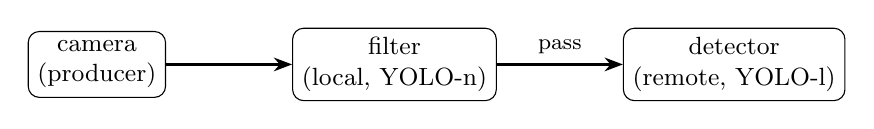
\begin{tikzpicture}[node distance=0.9cm and 1.6cm]
  \node[box] (cam) {camera\\(producer)};
  \node[box, right=of cam] (filter) {filter\\(local, YOLO-n)};
  \node[box, right=of filter] (det) {detector\\(remote, YOLO-l)};
  \draw[arrow] (cam) -- (filter);
  \draw[arrow] (filter) -- node[lbl] {pass} (det);
\end{tikzpicture}
\caption{Early discard. The engines run in series: the filter forwards a frame
to the remote detector only if it passes.}
\label{fig:early-discard}
\end{figure}

For each frame, the filter reports \code{Pass} if the frame should go to the
cloudlet, and \code{Stop} otherwise. It can also report its own detections as
a result. The filter only returns a verdict; the client still holds the frame
and sends it on (\S\ref{sec:forwarding}). Raising the filter's threshold as
bandwidth drops is the knob the paper uses for bandwidth adaptation.

The flow is a chain, so each frame keeps its token all the way to the end.
Suppose the camera produces 30 frames/s, the filter takes 0.1~s per frame, the
detector takes 0.3~s including the network, and the producer has $C = 1$
token:
\begin{itemize}[nosep]
  \item A discarded frame returns its token after the filter, at 0.1~s. A
        frame that passes keeps it until the detector finishes, at 0.4~s.
  \item In a scene with few targets, where 10\% of frames pass, the producer
        sends about $1/(0.1 + 0.1 \times 0.3) \approx 7.7$ frames/s. In a scene
        where every frame passes, it sends about 2.5 frames/s, which is what
        the cloudlet and the network can handle.
  \item Only frames that pass go over the network, and only while they hold
        a token. If the link slows down, these frames keep their tokens
        longer, and the producer slows down too.
  \item Camera frames the producer cannot send are skipped; each new token
        takes the newest frame.
\end{itemize}
While all tokens are held by frames at the cloudlet, the filter has nothing to
do. With $C > 1$, the filter keeps checking new frames while earlier frames are
at the cloudlet, at the cost of more frames in flight.

The app reads both engines' results from its producer's result service. The
\code{forward} field of the filter's \code{Result} tells it whether a detector
result may follow.

\subsection{Multi-tier fusion}
\label{sec:fusion}

\begin{figure}[h]
\centering
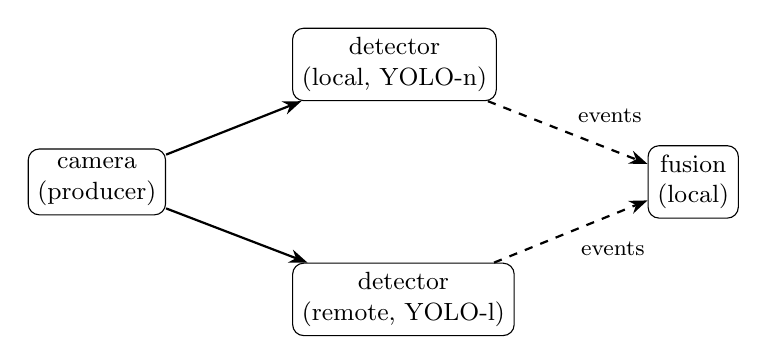
\begin{tikzpicture}[node distance=0.6cm and 1.6cm]
  \node[box] (cam) {camera\\(producer)};
  \node[box, above right=of cam] (local) {detector\\(local, YOLO-n)};
  \node[box, below right=of cam] (remote) {detector\\(remote, YOLO-l)};
  \node[box, anchor=west] (fusion) at ($(local.east)!0.5!(remote.east) + (1.8,0)$) {fusion\\(local)};
  \draw[arrow] (cam) -- (local);
  \draw[arrow] (cam) -- (remote);
  \draw[subscription] (local) -- node[font=\footnotesize, midway, above right] {events} (fusion);
  \draw[subscription] (remote) -- node[font=\footnotesize, midway, below right] {events} (fusion);
\end{tikzpicture}
\caption{Multi-tier fusion. Solid arrows are a flow; dashed arrows are
subscriptions to event services. Both detectors process the same frames in
parallel, and the fusion engine combines their results.}
\label{fig:fusion}
\end{figure}

The paper always runs on-device AI at the same time as cloudlet AI, instead of
falling back to on-device AI after a network timeout. The local result comes
early and can trigger a speculative action. The cloudlet result, when it
arrives, is definitive, and can confirm or cancel that action.

\paragraph{Flow control.} The camera feeds both detectors. Suppose the local
detector processes 10 frames/s and the remote one, including the network,
3 frames/s:
\begin{itemize}[nosep]
  \item Each frame's token returns at its first completion, which is usually
        the local detector's result. So the producer sends 10 frames/s, the
        rate of the fastest path.
  \item Whenever the remote detector is free, it takes the newest admitted
        frame, which the local detector has also received
        (\S\ref{sec:aligned}). So every frame processed remotely also has a
        local result, and fusion can match the two by \code{InputId}.
  \item The crossing to the remote server has a small capacity, so a slow
        link sends fewer frames, and the local detector is not affected.
  \item The cloudlet can be faster than the device, despite the network
        delay. Then the roles swap. If the faster side changes from frame to
        frame, some frames get only one result.
\end{itemize}

\paragraph{Fusion.} The fusion engine subscribes to the event services of both
detectors (\S\ref{sec:subscribe}). It is not part of the flow, so it never
slows the detectors down. It cannot count on getting both results for a frame, and does not
always need both: its own logic decides how long to wait for the remote
result. The result events tell it what can still come:

\begin{center}
\small
\begin{tabular}{@{}p{0.36\linewidth}p{0.3\linewidth}p{0.26\linewidth}@{}}
\toprule
Fusion has for a frame & Meaning & Fusion can \\
\midrule
local \code{Result}, remote \code{Sent}
  & a remote result may come & wait, up to its own limit \\
local \code{Result}, remote \code{Skipped}
  & the remote detector never got the frame & act on the local result now \\
remote \code{TimedOut}, \code{Disconnected}, or \code{Lost}
  & no remote result in time & act on the local result now \\
remote \code{Result} after its \code{TimedOut}
  & the definitive answer, after giving up & confirm or cancel its action \\
\bottomrule
\end{tabular}
\end{center}

The local \code{Result} usually arrives first and can trigger a speculative
action. The remote detector skips most frames. A frame in its pending slot can
still be taken after the local result arrives. Fusion finds out which happens
when the remote detector takes the frame (\code{Sent}), or when the next
admitted frame replaces it (\code{Skipped}). The next frame is admitted as
soon as the local detector finishes, so fusion knows within about one camera
frame whether to wait. A late remote result can still cancel a speculative
action that turned out to be a false positive. When the cloudlet is faster
than the device, the same table applies with local and remote swapped.

Fusion's waiting limit is separate from Gabriel's offer deadlines, which only
reclaim tokens and capacity; fusion can give up much earlier. Fusion publishes
its decisions as \code{Derived} results. Fusion can also be part of the
producer's app (e.g.\ the SteelEagle OS) rather than a separate engine; it then
reads the same events from \nolinkurl{gabriel/producer/<name>/result}.

\subsection{Feedback: PatchCore}
\label{sec:feedback}

\begin{figure}[h]
\centering
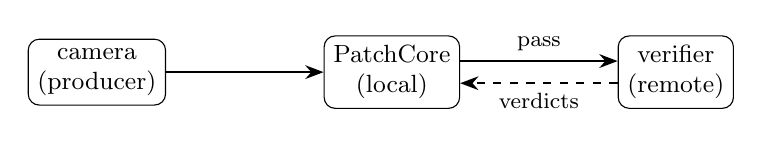
\begin{tikzpicture}[node distance=0.9cm and 2.0cm]
  \node[box] (cam) {camera\\(producer)};
  \node[box, right=of cam] (pc) {PatchCore\\(local)};
  \node[box, right=of pc] (ver) {verifier\\(remote)};
  \draw[arrow] (cam) -- (pc);
  \draw[arrow] ([yshift=4pt]pc.east) -- node[lbl] {pass} ([yshift=4pt]ver.west);
  \draw[subscription] ([yshift=-4pt]ver.west) -- node[font=\footnotesize, midway, below] {verdicts} ([yshift=-4pt]pc.east);
\end{tikzpicture}
\caption{Feedback. PatchCore forwards suspected anomalies to a remote
verifier in an early-discard flow, and subscribes to the verifier's event
service to update its memory bank.}
\label{fig:feedback}
\end{figure}

PatchCore scores each frame against its memory bank of normal patch features.
The flow is early discard, and PatchCore also subscribes to the verifier's
events:
\begin{enumerate}[nosep]
  \item For a normal frame, PatchCore reports \code{Stop}, and the token
        returns.
  \item For a suspected anomaly, PatchCore reports \code{Pass}, with its
        anomaly report as the result; the app can act on that report right
        away. PatchCore also caches the frame's patch features, keyed by
        \code{InputId}. The client sends the frame on to the verifier, and the
        frame keeps its token until the verifier completes it.
  \item The verifier reports its verdict as a \code{Result}. The remote server
        sends it to the client, which republishes it on the device on the
        verifier's event service.
  \item PatchCore reads the verdict from its subscription between frames. If
        it is a false positive, PatchCore adds the cached features to its
        memory bank. Either way, it removes the cache entry. It also removes
        entries whose verifier offer ended with \code{Skipped},
        \code{TimedOut}, or \code{Disconnected}, and older entries on
        \code{Lost}.
\end{enumerate}
Feedback does not change token accounting: the frame's token came back when
the verifier completed it, and subscriptions carry no tokens. PatchCore waits
for whichever comes first, an input or an event, with one call.

\paragraph{The cost of an update.} PatchCore processes frames and reads
verdicts in the same loop. An incremental update, appending the features and
adding them to the nearest-neighbour index, takes milliseconds and can be done
inline. A full rebuild of the memory bank can take seconds; PatchCore should
then hand it to a background thread and swap the new bank in when it is ready,
so that frames do not stall.

\subsection{Telemetry}
\label{sec:telemetry}

The client hosts \emph{internal producers} for its own measurements, such as
its bandwidth and round-trip estimates. They publish on ordinary iceoryx2
producer services, e.g.\ \nolinkurl{gabriel/producer/<client>.bandwidth/input},
and give their inputs ids like any producer. So any process can use them:
\begin{itemize}[nosep]
  \item the app or an engine can subscribe directly, e.g.\ to raise a filter's
        threshold as bandwidth drops, the paper's bandwidth adaptation;
  \item a flow can take them as its producer, when the consumer wants them
        rate-limited and newest-wins.
\end{itemize}

\subsection{Combining them}

One flow can use several patterns. For example, a filter can sit in front of
the remote detector, and a fusion engine can combine the filter's and the
detector's results. The detector then only receives frames the filter has
already processed, so alignment is automatic. Feedback can be added to either:
the filter can also subscribe to the remote detector's events.

\section{Disconnected operation}
\label{sec:disconnected}

This section is a planned extension: the first version does not need it, but
the design above leaves room for it.

\subsection{What already works}

Live flows keep running while the cloudlet is unreachable:
\begin{itemize}[nosep]
  \item Crossings to the remote server have no spare capacity while it is
        disconnected (\S\ref{sec:crossing}). Remote branches skip their
        inputs, while local engines keep processing at their own rate. In
        multi-tier fusion, fusion gets \code{Skipped} or \code{Disconnected}
        for the remote detector and acts on the local result.
  \item Inputs already on the remote server end with \code{Disconnected},
        their tokens come back, and the app learns which frames lost their
        remote results.
\end{itemize}
What live flows deliberately do not do is keep a backlog: a frame that cannot
be sent is skipped. Reintegration and reachback need the opposite: recorded
frames that are sent later and must not be lost. The design below supports
them without giving up skipping for live flows.

\subsection{The storage engine}

The paper keeps two logs in the device's non-volatile storage: a
\emph{DataLog} with every frame at full fidelity, and an \emph{OpLog} of
requests waiting to be sent to the cloudlet, ordered by mission-specific
priority. In Gabriel, both live in a \emph{storage engine}: a local process
that records frames and serves them back later. It plays two roles, in
different flows:

\begin{figure}[h]
\centering
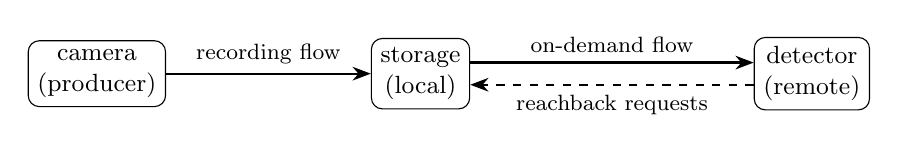
\begin{tikzpicture}[node distance=0.9cm and 2.6cm]
  \node[box] (cam) {camera\\(producer)};
  \node[box, right=of cam] (store) {storage\\(local)};
  \node[box, right=3.6cm of store] (det) {detector\\(remote)};
  \draw[arrow] (cam) -- node[lbl] {recording flow} (store);
  \draw[arrow] ([yshift=4pt]store.east) -- node[lbl] {on-demand flow} ([yshift=4pt]det.west);
  \draw[subscription] ([yshift=-4pt]det.west) -- node[font=\footnotesize, midway, below] {reachback requests} ([yshift=-4pt]store.east);
\end{tikzpicture}
\caption{The storage engine records frames in its own flow, and serves stored
frames to the cloudlet as an on-demand producer. Reachback requests reach it
through a subscription to the detector's event service.}
\label{fig:storage}
\end{figure}

\begin{itemize}[nosep]
  \item \textbf{An engine, in its own recording flow.} The camera feeds the
        storage engine on an ordinary input edge. The storage engine stores
        each frame under its \code{InputId} and capture time, and reports
        \code{Stop}.
  \item \textbf{An on-demand producer}, which publishes stored frames into
        on-demand flows that lead to cloudlet engines (below).
\end{itemize}
It uses the ordinary engine and producer ABIs, so it needs no special support.
Gabriel can ship a default storage engine, and a mission can replace it.

\paragraph{Why its own flow.} Writing a frame is fast, so the storage engine's
path would usually complete first. In a flow shared with other engines, the
producer would then admit frames at the storage engine's speed, and every
other engine would become a slow branch. That breaks alignment for fusion
(\S\ref{sec:aligned}): if the local and remote detectors are both slow
branches, each takes the newest frame from its own pending slot, and they often
process different frames. Each flow has its own token pool for the producer
(\S\ref{sec:tokens}), so in its own flow, the storage engine runs at its own
speed and does not affect the detection flows.

\paragraph{Losses.} The storage engine misses frames only when it cannot keep
up with the camera, as any recorder would. To absorb short stalls, e.g.\
while the disk flushes, its edge gets a capacity above 1 and its flow a few
tokens, so frames wait at the engine instead of being skipped.

\paragraph{Priorities.} Which stored frame to send next, and how priorities
change as old requests lose value, is mission logic. Requests carry a
priority, and the storage engine orders its OpLog by it; a mission can plug in
its own ordering.

\subsection{On-demand producers}

A live producer offers its newest frame whenever the client could admit it. An
on-demand producer turns this around: the client tells it when it \emph{could}
admit an input, and the producer then chooses what to publish.
\begin{enumerate}[nosep]
  \item The client sees that the flow's pool for the producer has a token and
        that one of the producer's edges can send right away: exactly the
        admission rule (\S\ref{sec:tokens}).
  \item It signals the producer that it is ready.
  \item The storage engine takes the most important entry from its OpLog
        \emph{at that moment}, and publishes the stored frame under the frame's
        \emph{original} \code{InputId}, the one the camera gave it. The
        cloudlet's record of completed inputs and the requesting engine can
        then match it.
  \item The client admits it, and from then on it is an ordinary input:
        tokens, offers, outcomes, and result events work as for live frames.
\end{enumerate}
Because the producer chooses only when there is room, priorities can change at
any time, and the most important request always goes next. Tokens still bound
how many stored frames are in flight, so reintegration over a weak link does
not flood it. While the cloudlet is unreachable, its crossings have no spare
capacity, the client never signals ready, and the OpLog simply grows. When the
connection returns, the signals resume and the OpLog drains in priority order.

Once admitted, an on-demand input is never replaced, because the client admits
it only when an edge can send it right away. Further along its path, a busy
edge can still skip it. An on-demand flow should therefore usually be a chain
to the remote engines, without fan-outs that would race it against other
branches.

\subsection{Reliable delivery}

The storage engine removes an entry from its OpLog only when the entry's
result arrives. Any other ending, \code{Skipped}, \code{TimedOut}, or
\code{Disconnected}, leaves the entry in the OpLog, so it is sent again the
next time it is the most important. The notification guarantee
(\S\ref{sec:events}) is what makes this safe: every offer of the input ends
with exactly one event, so the storage engine always learns whether to keep
the entry. It receives these events by subscribing to the event services of
the engines in its on-demand flows.

\subsection{Exactly-once processing at the cloudlet}

Retrying can send the same frame twice: a result may be lost with the
connection after the remote engine already processed the frame. The paper
requires each request to be processed only once. The remote server therefore
keeps, for on-demand flows, a bounded record of recently completed inputs and
their results, keyed by \code{InputId}. When an input arrives that is already
in the record, the server does not run the engines again; it reports the
recorded result instead. This relies on ids that stay the same across retries
and device restarts, which is why producers choose them (\S\ref{sec:ids}).

How long the record must last depends on how long a retry can take, which can
be the length of a disconnection. An open question is whether it must survive
a restart of the remote server, which would require keeping it on disk.

\subsection{Reachback}

In reachback, a cloudlet engine asks for specific recorded frames, e.g.\ the
frames around an abandoned vehicle where no person was detected. It needs no
new mechanism:
\begin{enumerate}[nosep]
  \item The engine reports its request as an ordinary result, or as a
        \code{Derived} result. It names the frames it wants by \code{InputId}
        or by capture time, which every frame carries, and gives the request a
        priority.
  \item The storage engine subscribes to that engine's event service
        (Figure~\ref{fig:storage}), which the client republishes on the
        device, so it receives the request. It adds the requested frames to
        its OpLog.
  \item As an on-demand producer, it sends them in an on-demand flow that
        leads to the requesting engine. They are delivered reliably and
        processed once, as above.
\end{enumerate}
The request format is between the requesting engine and the storage engine,
so Gabriel treats it as an ordinary result. A standard format can be added
later if several engines need it.

\subsection{Sharing the link}

Live and on-demand flows share the device's connection to the remote server.
While weakly connected, live frames should usually go first, and
reintegration should use what is left. QUIC supports this directly: each
stream has a priority, and quinn sends higher-priority streams first. Inputs
of live flows are sent on higher-priority streams than inputs of on-demand
flows. The priority of each flow can be part of its spec.

\subsection{Changes to the rest of the design}

\begin{itemize}[nosep]
  \item Producers choose input ids, and each frame carries its capture time
        (\S\ref{sec:ids}). The token pool takes the id from the input when admitting it,
        instead of making one.
  \item Result events carry their flow's name (\S\ref{sec:events}).
  \item Crossings to a disconnected server have no spare capacity
        (\S\ref{sec:crossing}).
  \item Producers can be on-demand, with a ready signal from the client, and
        can publish a frame under another producer's \code{InputId}.
  \item A storage engine, in its own recording flow, records frames and
        serves them back as an on-demand producer.
  \item The remote server keeps a record of completed on-demand inputs.
  \item Streams are prioritized by flow.
\end{itemize}

\section{Wire format}
\label{sec:wire}

The client speaks the same protocol to both servers; only the transport
differs. Control calls are encoded with postcard, and each carries the
\code{PROTOCOL\_VERSION} it was made with; a server refuses a call of another
version. On one machine, inputs and events have fixed-size records instead
(\S\ref{sec:services}). Over QUIC, every message will be encoded with
postcard.
\begin{itemize}[nosep]
  \item \textbf{Control calls} (client to server): \code{InstallFlow}, which
        carries the server's part of a flow, and \code{RemoveFlow}. The server
        checks its part, and replies with success or an error.
  \item \textbf{Inputs} (client to server): an \code{InputHeader}, followed
        by the input's data. The server does not reply to an input. Instead,
        it reports what happens to the input as result events.
  \item \textbf{Result events} (server to client): one ordered stream of
        \code{ResultEvent}s for all of the server's engines. Using one stream
        guarantees that a parent's event arrives before its children's
        (\S\ref{sec:accounting}). The client republishes the remote server's
        events on the device's event services (\S\ref{sec:subscribe}).
\end{itemize}
\begin{lstlisting}
struct CrossingHeader {
    kind: CrossingKind,     // Input, or Skipped: a notice with no payload
    flow: u64,              // the session the server gave the flow at install
    offer: OfferId,         // its edge is the crossing; the server knows its targets
    input: InputId,
    payload_type: String,   // how to read the input's bytes
}
\end{lstlisting}
The receiver checks the length against the bytes it actually received, as the
client does with the iceoryx2 envelope today.

\paragraph{Point to data instead of carrying it.} On one machine, a message
that sends an input to a process or an engine points to the input's data
instead of containing it:
\begin{lstlisting}
struct DataRef { service: String, seq: u64 }
\end{lstlisting}
At first, the sender copies the data into a service of its own and points to
that copy. With zero copy (\S\ref{sec:data}), it points to the service where
the data was first written. Only inputs sent to the remote server carry the
bytes themselves.

\paragraph{Remote server: QUIC (quinn).} Each client has one connection. Each
control call uses its own bidirectional stream. Each input uses its own
unidirectional stream, which the client finishes after the input's bytes.
Result events use one long-lived unidirectional stream. Messages are
length-prefixed. An input stream carries a \code{CrossingHeader} and then the
input's bytes, up to the end of the stream; the server reads at most
\code{MAX\_INPUT\_SIZE} bytes. A skip notice is a stream with a header alone.
Input streams of live flows have a higher priority than
those of on-demand flows (\S\ref{sec:disconnected}). The threads that use the
connection are in \S\ref{sec:remote}. When the connection is
lost, the client reports
\code{Disconnected}, which ends every offer on the remote server. The remote
server removes the flows that client installed, which frees the capacity of
their edges. The client installs them again when it reconnects.

\paragraph{Local server: iceoryx2.} Clients find the local server by its
name.
\begin{itemize}[nosep]
  \item \textbf{Control calls} use request-response on
        \nolinkurl{gabriel/server/<name>/control}. The server answers calls
        each time its thread wakes, so within 10\,ms. iceoryx2 signals no
        event for a reply, so the client checks for it every 1\,ms, for up to
        1\,s. Calls are rare, so this costs little.
  \item \textbf{Inputs}: the client copies each input it sends on a crossing
        into a sample of \nolinkurl{gabriel/server/<name>/input}, with a
        \code{CrossingHeader}, and signals
        \nolinkurl{gabriel/server/<name>/input-ready}, which wakes the
        server. Skip notices (\S\ref{sec:crossing}) go the same way, as a
        header of kind \code{Skipped} with no payload.
  \item \textbf{Events}: the server publishes the events of a client's flows
        on \nolinkurl{gabriel/client/<client>/events}, numbered from 1, and
        signals \nolinkurl{gabriel/client/<client>/events-ready}. Each client
        has its own stream, so it reads only its own events, and a slow client
        fills only its own buffer.
\end{itemize}
If the local server dies, the client reports \code{Disconnected} for it, as
for the remote server, and installs its flows again when the server is back
(\S\ref{sec:client-thread}).

\paragraph{On each machine: iceoryx2.} Producers publish on
\nolinkurl{gabriel/producer/<name>/input}, with a ready event. The client
publishes result events for each producer's app on
\nolinkurl{gabriel/producer/<name>/result}. Each server sends inputs to its
engines, receives their outcomes, and publishes each engine's events, on
services under \nolinkurl{gabriel/engine/<name>/}. This works the same way
on both servers.

\subsection{Services on one machine}
\label{sec:services}

Seven iceoryx2 services carry an input from its producer to an engine and the
result back to the producer's app. Each is a publish-subscribe service. The sample's user header is
a fixed-size record, and its payload is a slice of bytes. Event services
(``Wake-ups'' below) only signal that a sample is there.

\begin{center}
\small
\begin{tabular}{@{}p{0.17\linewidth}p{0.2\linewidth}p{0.2\linewidth}p{0.33\linewidth}@{}}
\toprule
Service & From $\to$ to & Header & Payload \\
\midrule
Producer input (\code{.../input})
  & producer $\to$ client
  & session, sequence number, length, flow
  & the frame \\
Server input (\code{.../input})
  & client $\to$ local server
  & input or skip notice, the flow's session on the server, the client's
    offer on the crossing, the input id, the payload type
  & the input's bytes; none for a notice \\
Engine input (\code{.../input})
  & server $\to$ engine
  & the offer, the input id, the payload type
  & the input's bytes \\
Engine outcome (\code{.../outcome})
  & engine $\to$ server
  & the offer, the input id, what it forwards, the types of the result and
    of the new input, and the length of each
  & the new input of an \code{Emit}, then the result \\
Engine events (\code{.../events})
  & server $\to$ subscribers
  & the sequence number, the kind, the offer (none for \code{Derived}), the
    input id, the engine, the flow, what it forwards, the offers it created,
    the payload type
  & the result, if any \\
Client events (\code{.../events})
  & local server $\to$ client
  & as for engine events, numbered per client
  & the result, if any \\
Producer results (\code{.../result})
  & client $\to$ the producer's app
  & as for engine events, numbered per producer
  & the result, if any \\
\bottomrule
\end{tabular}
\end{center}

\paragraph{Wake-ups.} An iceoryx2 event service goes with each service whose
reader sleeps, so no side polls. After it delivers an input, the server
signals the engine's \code{.../input-ready}, which ends the engine's
\code{wait}. After it reports an outcome, the engine signals
\code{.../outcome-ready}, which ends the server thread's wait
(\S\ref{sec:server-thread}). After it sends an input, a client signals the
server's \code{.../input-ready}, which has one notifier per client. After it
sends a client events, the server signals the client's
\code{.../events-ready}. After it publishes events about a producer's inputs,
the client signals the producer's \code{.../result-ready}, which ends a
subscriber's \code{wait}; the server signals an engine's
\code{.../events-ready} the same way. A signal always follows the samples it announces, so
a woken side finds them.

\paragraph{Node names.} An engine's iceoryx2 node is named
\code{gabriel/engine/<name>}, a server's \code{gabriel/server/<name>}, and a
client's \code{gabriel/client/<name>}.
The server finds the process of each of its engines by this name
(\S\ref{sec:server-thread}).

\paragraph{Why the outcome goes through the server.} An engine's outcome is
not yet a result event. The server first frees the edge the offer was on, and
creates the offers that follow when the engine forwards the input. Only then
can it write the event, which lists those offers as its children
(\S\ref{sec:accounting}). So engines never publish events themselves. Each
event service has exactly one publisher: the server for its own engines, or
the client for the remote engines whose events it relays. That gives the
events of an engine one order. It also makes the engine's side identical on
both servers, because the client cannot read a cloudlet engine's services
directly.

\paragraph{The result comes last in an outcome.} An engine writes the new
input of an \code{Emit} in place, into a sample it loaned, and learns its
result only when it reports the outcome. Putting the result after the input
means nothing has to move.

\paragraph{Sequence numbers.} The publisher of an event service numbers its
events from 1. A subscriber that sees a number it did not expect knows how
many events it lost, and reports \code{Lost}. A subscriber can start in the
middle of the stream, so it takes the first number it sees as its start.

\paragraph{Fixed-size records.} A record must have a fixed layout so another
process can read it in place. So names are bounded strings, and lists have a
named maximum: the number of offers one event creates. A flow that exceeds a maximum is rejected when it is installed.
Engine names must be unique on a machine, because an event service is named
after its engine and has one publisher.

\paragraph{Payload types.} Gabriel treats a result as bytes, and does not
parse it. Each result carries a payload type, such as a protobuf message name,
so that a subscriber knows how to read it. For example, a storage engine that
subscribes to a local and a remote detector tells them apart by the engine
named in each event, and decodes each result by its payload type. The two
detectors need not use the same type.

\paragraph{Buffers.} iceoryx2 fixes a service's buffer sizes when the service
is created, and by default it overwrites the oldest sample when a buffer is
full. Each service sets this explicitly:
\begin{itemize}[nosep]
  \item \textbf{Inputs and outcomes are never dropped.} A dropped input or
        outcome would leave an offer open for ever. So both services turn
        overwriting off. Both buffers have the same small, fixed size, larger
        than the one input the server delivers to an engine before its
        outcome arrives (\S\ref{sec:edges}). With that bound, neither buffer
        can fill. If a bug broke the bound, iceoryx2 would by default wait
        until the receiver makes room, and the sender would hang. So both
        publishers install a backpressure handler that drops the sample and
        makes the send fail instead (\code{DiscardDataAndFail}). A failed
        input is lost (\S\ref{sec:server-router}); a failed outcome is an
        error for the engine, which can still take its next input.
  \item \textbf{Inputs from clients are never dropped} either. The server
        reads them all each time a client wakes it, so its buffer of 64 fills
        only while the server is stuck. Then a client's send fails, as above,
        and the input's crossing offer times out at the client.
  \item \textbf{A client's events drop the oldest}, with a buffer of 1024
        events. Every event matters to the client's token accounting, so the
        buffer is large, and the client can see a gap in the numbers
        (\S\ref{sec:gaps}).
  \item \textbf{Events drop the oldest}, on engines' event services and
        producers' result services alike. A subscriber that falls behind loses
        its oldest events and learns about it as \code{Lost}
        (\S\ref{sec:subscribe}). An event service accepts a fixed number of
        subscribers on its machine; remote clients get events over QUIC, so
        they do not count.
\end{itemize}

\paragraph{One input at a time.} The engine library gives its engine one
input, and expects one outcome for it, before it gives the next. No input waits
in the engine's input service, because the server delivers the next input
only when an outcome frees the engine's place (\S\ref{sec:edges}). A place is
also freed when an input is lost
(\S\ref{sec:server-router}), but such an input is not in the buffer: it never
arrived, its outcome came already, or the engine is dead.

\paragraph{The flow of each event.} One input can enter several flows under
the same \code{InputId}, so every event names its flow. A late result is not
marked: a reader that already saw its offer end knows that it is late.

\section{Logging}
\label{sec:logging}

Gabriel logs with the \code{tracing} crate. As a library, it only emits
events; the app decides whether and where they go. A Rust app installs any
\code{tracing} subscriber. A C app calls \code{gabriel\_log\_init}, which
prints to standard error, with a filter in the syntax of \code{RUST\_LOG}
(e.g.\ \code{"info"}); by default it prints warnings and errors.
\begin{itemize}[nosep]
  \item \textbf{Warnings}: every failure the server and client threads carry
        on after, e.g.\ a failed delivery, a malformed outcome, a refused or
        failed send, an event that could not be published; an engine that
        stopped; a lost connection to the local server.
  \item \textbf{Info}: engines served, flows added, installed, removed, and
        installed again after a lost connection.
  \item \textbf{Debug}: a flow the server refused, a failed attempt to
        install a flow again, and dropped events (duplicates, or events for
        offers that already ended).
  \item \textbf{Errors}: a server or client thread that stopped.
\end{itemize}
Each thread's events carry its server's or client's name. Nothing is logged
per input; the result events carry the per-input timestamps instead
(\S\ref{sec:events}).
The server and client steps return only their first error, so when several
fail at once, one warning stands for them.

\section{ABI changes}

\begin{itemize}[nosep]
  \item Engines receive the \code{InputId}, the payload type, and the bytes of
        each input. They report one outcome per input: \code{pass}, \code{emit}, or \code{stop}, each with
        an optional result. This replaces \code{publish\_result(producer,
        ...)}, which identified the input only by its producer.
  \item An engine says how to read its results with a payload type, given
        once when it is created. When it emits, it also names the type of the
        new input. Result events carry the type
        (\S\ref{sec:services}).
  \item Any process can subscribe to an engine's event service, and poll it
        for events. An engine gets a call to publish a \code{Derived} result
        for an \code{InputId}. An engine can also own subscriptions
        (\code{gabriel\_engine\_subscribe}): \code{gabriel\_engine\_wait}
        then ends for an input or an event of any of them, so that it does not
        have to poll both in a busy loop, and
        \code{gabriel\_engine\_poll\_event} returns the events, taking turns
        between the subscriptions. Each event names its engine; so does
        \code{LOST} on a subscription to an engine. The engine owns its
        subscriptions, rather than waiting on separate handles, because each
        handle stays on one thread.
  \item \code{add\_flow(name, spec)}: \code{spec} describes the nodes (local
        or remote), each producer's token count $C$, and the input edges with
        their engines' timeouts. The client rejects forbidden edges, and
        installs each part of the flow on its server. In C, \code{spec} is
        TOML (\S\ref{sec:install}); in Rust, it is a \code{FlowSpec}.
  \item \code{gabriel\_log\_init(filter)} prints Gabriel's log to standard
        error, for C apps (\S\ref{sec:logging}).
  \item Both servers are created with the same call. A server can always be
        reached by name over iceoryx2. If it is given an address to bind, it
        can also be reached over QUIC; until QUIC exists, an address is
        rejected, and \code{bind\_addr} must be NULL.
  \item The producer's app reads result events from
        \nolinkurl{gabriel/producer/<name>/result} with a subscription:
        \code{gabriel\_subscribe\_producer}, then
        \code{gabriel\_subscription\_wait} and
        \code{gabriel\_subscription\_poll}. A polled event stays valid until
        the next poll. Besides the published kinds, a poll can return
        \code{LOST}, with the number of events lost. Each event carries its
        timestamps in nanoseconds (\S\ref{sec:events}). A subscription to an
        engine's event service, made with \code{gabriel\_subscribe\_engine},
        uses the same calls.
  \item Producers stamp each frame with its \code{InputId}. A live producer
        does this automatically, and \code{publish\_input} returns the id (in
        C, its sequence number), so the app can match events to its frames,
        and note when it captured and published each. An on-demand producer gets a
        call that waits until the client is ready for an input, and publishes
        a frame under an id the app supplies.
  \item A flow's spec says whether each producer is live or on-demand, and
        gives the flow's priority on the network.
\end{itemize}

\section{Implementation plan}

Both servers run the same code, and the local server needs no networking. So
all the DAG logic can be built and tested on one machine first. The client's
receive thread, which subscribes to producers and keeps the newest input from
each, became part of the client thread (\S\ref{sec:client-thread}).

\begin{enumerate}[nosep]
  \item Edge capacities and pending slots, shared by the client and the
        server, and tickets with end-to-end tokens in the client. Unit tests
        cover every row of the token table, several completions, duplicates,
        late events, the admission rule, alignment at a fan-out, and the
        invariant.
  \item The server, with engines over iceoryx2, and the engine ABI with
        \code{Pass}, \code{Emit}, and \code{Stop}.
  \item The client-server protocol over iceoryx2, to the local server. Flows
        through local engines work end to end, e.g.\ a filter in front of a
        second local engine.
  \item Result events back to producers, including \code{Sent},
        \code{Skipped}, \code{TimedOut}, and \code{Disconnected}. Tests check
        that every offer ends with exactly one of them (done for the local
        server).
  \item The wire format: encoding and decoding every message with postcard
        (done for control calls, in step 3),
        with tests.
  \item The same protocol over QUIC, to the remote server
        (\S\ref{sec:remote}), in this order:
        \begin{enumerate}[nosep]
          \item a trait over the client thread's server link and one over
                the server thread's clients, with the local ones behind them
                and no change in behavior;
          \item the network thread, with control calls, inputs, skip notices
                and events over QUIC, tested over loopback (done; the client
                does not use it until the next step);
          \item the compiler accepts remote engines, splits a flow between
                the servers, gives remote crossings a configured capacity, and
                adds the round-trip bound to deadlines. Early discard works end
                to end (done);
          \item the bench runs the remote side in a network namespace with
                netem, and \code{analyze.py} reports the uplink, the return
                trip, and the AoI at the app (done).
        \end{enumerate}
  \item Event services and subscriptions, waiting for inputs and events
        together, \code{Derived} results, and the client's telemetry producer.
        Multi-tier fusion and feedback work end to end. In this order:
        \begin{enumerate}[nosep]
          \item subscriptions to an engine's event service on its own
                machine, woken after each batch of events (done);
          \item the client republishes the remote engines' events on the
                device (done);
          \item an engine subscribes to event services itself, and its
                \code{wait} ends for an input or an event of any of them
                (done);
          \item \code{Derived} results, sent by the engine to its server on a
                service of their own, since outcomes are limited to one in
                flight. The server publishes them on the engine's event
                service, and the remote server also sends them to its client.
        \end{enumerate}
        The telemetry producer comes after these.
  \item Crossings with several targets on one server.
  \item On-demand producers, the record of completed inputs on the remote
        server, and stream priorities: prioritized reintegration and
        reachback work end to end, including retries after a disconnection.
  \item Zero copy on one machine (\S\ref{sec:data}), if measurements show
        that the copies matter.
\end{enumerate}

\section{Known gaps}
\label{sec:gaps}

A review of the design against its goals and failure modes found the gaps
below. None needs a new mechanism: each is fixed by ending offers the way the
design already does, with \code{TimedOut} or \code{Disconnected}, or by
detecting gaps in sequence numbers or dead iceoryx2 nodes.

\subsection{Gaps in the goals}

Two gaps in the goals were found and are now closed:
\begin{itemize}[nosep]
  \item \textbf{Skips at the client reach engines' subscribers} (goal 6). An
        input can be skipped in a crossing's pending slot, on the client, and
        fusion must learn it (\S\ref{sec:examples}). For a local engine, the
        client sends the local server a skip notice, and the server publishes
        \code{Skipped} on each target engine's event service
        (\S\ref{sec:crossing}). For a remote engine, the client relays the
        remote server's events, so it will publish its own \code{Skipped}
        there too.
  \item \textbf{The local event stream to the client may lose events} (goals
        4 and 6). Over iceoryx2, blocking would let a slow client stall the
        server, so the stream drops its oldest events when the client falls
        behind. The stream numbers its events and has a large buffer, and the
        client treats a gap in the numbers like a lost connection: it reports
        \code{Disconnected}, which ends every offer on the server, and installs
        its flows again (\S\ref{sec:client-thread}).
\end{itemize}

The first benchmark runs (\code{docs/evaluation.tex}) found a third, which
needs no new mechanism:
\begin{itemize}[nosep]
  \item \textbf{Too few tokens freeze a pending slot} (goal 2: slow engines
        should skip to the newest frame). When the input in an engine's
        pending slot holds the producer's last token, no newer input can
        replace it, and it waits for the rest of the engine's time. One more
        token fixes it: newer inputs then replace it, and its token comes
        back with \code{Skipped}. The server owns the slot and decides, so no
        change to the protocol is needed, only a rule for $C$ (``Choosing
        $C$'' in \S\ref{sec:tokens}).
\end{itemize}

\subsection{Failure modes}

\begin{center}
\small
\begin{tabular}{@{}p{0.24\linewidth}p{0.33\linewidth}p{0.35\linewidth}@{}}
\toprule
Failure & Now & Extension \\
\midrule
Engine hangs
  & Its offers time out. It gets no new inputs, because delivered inputs keep
    their places. & --- \\
Engine dies
  & Noticed within a second by its node (\S\ref{sec:server-thread}). Its
    delivered offers end with \code{TimedOut}, its pending offers with
    \code{Skipped}, and its places are freed (\code{engine\_lost}).
  & --- \\
Engine not started, or delivery fails
  & The input is lost: its offer ends with \code{TimedOut} at once and its
    place is freed (\code{input\_lost}). & --- \\
Outcome is malformed
  & Reported as an error; the input is lost, as above. & --- \\
Engine reports another engine's offer, or an offer twice
  & Ignored: the router acts on an outcome only for an input it delivered to
    that engine and that has no outcome yet. & --- \\
Local server dies or restarts
  & Noticed within a second by its node (\S\ref{sec:client-thread}). Every
    offer on it ends with \code{Disconnected}, and the client installs its
    flows again once the server runs. Outcomes from before the restart find
    no flow and are ignored; the new random session keeps offer ids apart.
  & --- \\
Local client dies
  & A client that stops removes its flows. One that crashes leaves them
    installed on the local server.
  & The server already records which client installed each flow. It would
    remove them when that client's node dies, as a remote server will when
    the QUIC connection closes. \\
A buffer that must not overflow is full
  & Cannot happen while the delivery bound holds. If a bug breaks the bound,
    the send fails instead of waiting (\S\ref{sec:services}). & --- \\
Errors inside the server or client
  & Handled as above, and logged as warnings (\S\ref{sec:logging}).
  & --- \\
Network lost or slow
  & Designed: \code{Disconnected}, crossings keep only their newest input,
    flows are installed again on reconnect. & Adjusting crossing capacities,
    later. \\
Subscriber falls behind
  & It loses the oldest events and learns it as \code{Lost}. & --- \\
Clocks
  & Gabriel's logic compares no clocks across machines. Measurements that
    do use the client's receipt stamps, and later an offset estimate
    (\S\ref{sec:remote}). & Offset estimate, later. \\
\bottomrule
\end{tabular}
\end{center}

\section{Open questions}
\label{sec:open}

\begin{itemize}[nosep]
  \item Whether the token rule (``Choosing $C$'' in \S\ref{sec:tokens})
        holds with the remote server, where the knee includes the network
        round trip, once each remote crossing adds its capacity to the
        count. With sections, the round trip is part of $Z$ instead.
  \item \textbf{Changing a flow at runtime} (later). Control calls block the
        client thread until the reply, which costs a round trip to the remote
        server each time a flow is installed. That is fine while flows are
        installed once; if they change often, calls should return at once,
        with replies read like events. Changing only the remote part could
        then install the new part, switch the crossings to it, and remove the
        old part once its offers ended; removing a flow would first have to
        end its open offers with events, so their tokens come back. Moving an
        engine between the device and the cloudlet also changes the client's
        router, whose open tickets must drain or move.
  \item The values of \code{IDLE\_TIMEOUT}, \code{KEEP\_ALIVE\_INTERVAL} and
        \code{REMOTE\_RTT\_BOUND} (\S\ref{sec:remote}), and whether the
        offset between the clocks is worth estimating in Gabriel or only in
        the analysis.
  \item The starting capacity of a crossing to the remote server, and how the
        client adjusts it from the measured wait and idle time
        (\S\ref{sec:alternatives}). A
        capacity of 3 or more keeps the remote pending slots fresh, but sends
        every admitted input over the network; less saves bandwidth, but the
        remote engine may start on inputs one processing time old
        (``Freshness'' in \S\ref{sec:edges}).
  \item Whether some engines should get a second input ahead of time, as an
        option. An engine that runs in microseconds loses throughput to the
        idle gap after each outcome; the inference engines Gabriel targets do
        not.
  \item The ticket deadline, and the deadline of an offer in flight. An input
        stops being forwarded once its ticket is past its deadline, so the
        ticket deadline should cover the offer deadlines along the longest path
        of the flow. The compiler now computes both from the engines' timeouts
        (\S\ref{sec:install}). They are upper bounds: an input that is lost
        holds its token until then. Whether tighter bounds are worth it is
        open.
  \item The default buffer size of a subscription to an event service.
  \item \textbf{Several clients of one remote server} (later). For now, a
        remote server has one client. With several, the server must choose
        which clients get an engine's \code{Derived} result, which names only
        a flow and an input; and two clients on one device that relay the
        same remote engine would both publish its event service.
  \item \textbf{Sections} (planned, \S\ref{sec:sections}). Open:
        \begin{itemize}[nosep]
          \item An input that the fast branch skipped, but that is alive on
                a slow branch, holds R's token until the slow branch
                completes it. With a tight count, this slows the producer.
                The second condition of admission makes it rare; how rare,
                with jitter, needs measuring.
          \item An engine shared by several flows or edges serves each of
                them more slowly than its own time. $S_k$ from \code{Sent} to
                \code{Result} misses that; the gap between a flow's results
                at the engine may be the better measure.
          \item The constants, to tune by measurement. The shadow run used
                a gain of 1/8 for \code{SERVICE\_TIME\_GAIN}, 10 for
                \code{MIN\_SAMPLES}, 0.1 for \code{ROUNDING\_TOLERANCE},
                and 0.05 for \code{COUNT\_HYSTERESIS}.
          \item Fan-outs, which the simulation does not cover yet: how
                often a result waits at a fan-out because no branch has a
                token, and what that costs F.
          \item Large inputs on a crossing. $Z$ counts the round trip, not
                the time to send the input's bytes; at low bandwidth, that
                time should be added from the bandwidth estimate.
          \item Branches that leave their server, to the client or over a
                crossing. Their completions are seen only by the client, so
                their pools would have to live there, at the cost of a round
                trip per gate.
          \item A slow network link as the bottleneck. $D_{\max}$ counts
                engines only; the crossing capacity limits the link, as
                today.
          \item Engines whose results the app reads, in the middle of a
                chain. Gating them also lowers how many results the app
                gets.
          \item Joins, once they exist. A join that needs results from
                both branches makes the fork-to-join region one section,
                whose branches take an input all together or not at all.
          \item Predictive pull, which would turn a count into a time.
        \end{itemize}
  \item \textbf{Pending slots holding more than one input.} Sections
        (\S\ref{sec:sections}) plan queues in order inside a section, bounded
        by its tokens. Outside sections, for streams where every input
        matters, such as audio chunks, a pending slot could keep the last $k$
        inputs and deliver them oldest first, dropping the oldest when full.
        This trades freshness for fewer skips, so the default stays 1.
  \item The buffer size of the local event stream to the client, and how
        often a gap in it is acceptable before it costs too much to install
        the flows again (\S\ref{sec:gaps}).
  \item Which encoding apps are expected to use for results. Gabriel only
        carries bytes and a payload type, so protobuf is a convention. An
        engine that returns results of several types would need the type per
        call, not per engine.
  \item The maximum number of offers created by one event, and the number of
        inputs a server delivers to an engine before their outcomes arrive.
        Both are constants, because iceoryx2 fixes record and buffer sizes
        when a service is created, and flows come and go at runtime. Their
        values are guesses to tune by measurement.
  \item Join nodes, which combine several inputs (e.g.\ a frame and a GPS
        reading) into one output.
  \item Flows that span several remote servers.
  \item Whether the remote server should keep a device's flows for a while
        after a disconnection, since short disconnections are common in DDIL
        settings.
  \item How long the remote server keeps its record of completed on-demand
        inputs, and whether it must survive a restart of the server.
  \item Whether a standard format for reachback requests is worth adding.
\end{itemize}

\end{document}
